\documentclass{article}

\usepackage{import}
\usepackage{pdfpages}
\usepackage{transparent}
\usepackage{indentfirst}
\usepackage[paper=a4paper, top=2.5cm, bottom=2.5cm, left=2.5cm, right=2.5cm]{geometry} 
\newcommand{\incfig}[2][1]{%
    \def\svgwidth{#1\columnwidth}
    \import{./figures/}{#2.pdf\_tex}
}  

% https://tex.stackexchange.com/questions/141569/highlight-textcolor-and-boldface-simultaneously
\usepackage{xcolor}
\usepackage{color, soul} 
\usepackage{tcolorbox}  % Creating colored boxes  
\counterwithin{table}{section}    

% Add a subsubsubsection 
\newcommand{\subsubsubsection}[1]{\paragraph{#1}\mbox{}}
\setcounter{secnumdepth}{4}
\setcounter{tocdepth}{4}

% Code 
\usepackage{listings}   
\definecolor{dkgreen}{rgb}{0,0.6,0}
\definecolor{gray}{rgb}{0.5,0.5,0.5}
\definecolor{mauve}{rgb}{0.58,0,0.82}

\lstset{frame=tb,
    language=java,
    aboveskip=3mm,
    belowskip=3mm,
    showstringspaces=false,
    columns=flexible,
    basicstyle={\small\ttfamily},
    numbers=none,
    numberstyle=\tiny\color{gray},
    keywordstyle=\color{blue},
    commentstyle=\color{dkgreen},
    stringstyle=\color{mauve},
    breaklines=true,
    breakatwhitespace=true,
    tabsize=3,
}  

\pdfsuppresswarningpagegroup=1 

\title{Android study}
\author{Juliane Marubayashi}
\date{ 2022-04-19 } 


\begin{document}
    \maketitle
    \newpage
    \tableofcontents
    \newpage
    \textbf{Attention before reading}: this document is not original. It is deeply based on the resources.
    Thus, I don't have any credit on the biggest part of this text. 
    \section{Lecture 1 - Basic Android}
    The android framework for building applications was developed in C and wrapped in java. 
The java virtual machine was also written in C and optimized for small devices and cores. 
The framework itself was based in reuse and extension patterns.   

The \textbf{application framework} is a \textbf{high level library in java} suitable to the creation
of user android applications. In other words, it's the basic structure underlying the system (Android API).  
The framework also creates the higher-level Android management services (Java).  

\begin{itemize}
    \item Activity manager
    \item Content manager 
    \item Resource manager 
    \item Location manager 
    \item Notification manager
\end{itemize}

\subsection{Application components}
The android applications can contain serveral independent components:  
\begin{itemize}
    \item Activities 
    \item Services 
    \item Broadcast Receivers 
    \item Content providers 
\end{itemize}

\subsubsection{Activities}
\begin{itemize}
    \item Contain a portion of the user interface
    \item Execute a well-defined task inside the application 
    \item Are subclasses of the android.app.Activity class
    \item Are usually composed by a hierarchy of Views
\end{itemize}

\subsubsection{Services}
\begin{itemize}
    \item Don't have user interface, like the activities
    \item Can execute in background for indeterminate period
    \item It's possible to estabilish a connection with the service and communicate through a
    well-defined programming interface
\end{itemize}

\subsubsection{Broadcast}
It handles notifications and the applications react to then. 
\begin{itemize}
    \item Can receive and react to notification received from the system or other applications 
    \item Applications can initiate a notification 'broadcast' 
\end{itemize}

\subsubsection{Content providers} 
Basically allow the comunication of data between applications.
\begin{itemize}
    \item Make available to other applicationo a data collection maintaned by this application
    \item Define an interface to access, add and update the supported data types
\end{itemize}

\subsection{Component activation}

\subsubsection{Activities and Services}
\hl{Activities and services are activated through an \textbf{Intent}.}

The \textbf{intent} identify the component or specify actions for activities and services.  

A explicit intent contains the:
\begin{itemize}
    \item Class reference of the desitnation
    \item Specification of an action, category, data (in the form of url) and possibly extra information.
\end{itemize}

Once the specifications are given, the android will try to find a matching component capable of executing ht eaction in the data (or data type) specified.
When activities and services are declared in the \textbf{manifest} they can specify the \textit{intent-filters}, describing their accepting intents.

An example is calling the activity using an intent:
\begin{lstlisting}
val otherActivity: Intent = Intent(thisActivity, OtherActivity::class.java);
thisActivity.startActivity(otherActivity);
\end{lstlisting}

\subsubsection{Broadcast receivers}
The intents for activating broadcast receivers indentify a \textbf{message} to be delivered to matching receivers.
The message is specificied using: action, category, data and extra info.

\begin{lstlisting}
sendBroadcast(Intent);      // Sends the intent.
onReceive(Context, Intent); // If a broadcast receiver was installed and matches the intent, this method will be called.
\end{lstlisting}

\subsubsection{Content providers}
When declared in the manifest must have an 'authority'. The 'authority' must recognize a name for 
its data collection. 

The content providers supports the CRUD operations on the specified collection. 

They are usually activated by the method \textbf{getContentResolver} and the \textbf{ContentResolver} can
insert, update, delete and query an information.

\begin{lstlisting}
ContentResolver resolver = getContentResolver();
Uri uri = Uri.parse("content://<authority>/<data-collection>[/<item>]"); 
resolver.query(Uri uri, String[] projection, Bundle queryArgs, CancellationSignal cancellationSignal);
resolver.delete(Uri uri, Bundle extras); 
resolver.insert(Uri uri, ContentValues values);
resolver.update(Uri uri, ContentValues values, Bundle extras);
\end{lstlisting}

\subsection{Intent (start an activity example)}

All the intents have a name (action) and can gave nire data associated (e.g uri, category, extra info). 

\hl{The intents can also be \textbf{explicit} with a class reference (inside an app).}

There're many predefined intents. 

This first example matches the android activity in the Dialer application, that allows the 
user to make a phone call, declared in an intent-filter, that can handle this action.

\begin{lstlisting}
val intent = Intent(Intent.ACTION_DIAL);
startActivity(intent);
\end{lstlisting}

This second example, matches an activity that makes a phone call, but for a given number.
\begin{lstlisting}
val intent = Intent(Intent.ACTION_CALL);
Uri.parse("tel:555-555-555").also{intent.date = it};
startActivity(intent); 
\end{lstlisting}

Creating an intent to start an activity externally the app: 
\begin{lstlisting}
Intent LaunchIntent = getActivity().getPackageManager().getLaunchIntentForPackage(CALC_PACKAGE_NAME);
startActivity(LaunchIntent);
\end{lstlisting}


\subsubsection{Intents data}
\hl{Intents \textbf{can transport data between components}}. In other words, if the application is currently running in an activity,
we can initiate another activity and parse the actual information to it by using intents. 

The \textbf{data} property can be used for any kind of a Uri. The calling and new app components uses the Intent \textbf{data} property
of the Uri type, by calling \textbf{setData()} and \textbf{getData()} methods to set it. 

The Extra internal field is used for arbitrary data types. 

It is a \textbf{Bundle} : set of (name, value) pairs organized in a hash table.
\begin{itemize}
    \item The value can be a String, simple type, or an array.
    \item Can also be any Serializabe or Parcelable (more efficient) object
    \item The values are inserted with some \textbf{putExtra(String name, ... value)} method and retrieved
    with \textbf{get...Extra(String name)}.
\end{itemize}

\begin{lstlisting}
override fun onCreate(savedInstanceState: Bundle?){
    super.onCreate(savedInstanceState);
    ...
    /* Activities have an intent property */ 

    val fName = intent.getStringExtra("firstName");
    val lName = intent.getStringExtra("lastName");
}
\end{lstlisting}

\begin{tcolorbox}[colback=red!5,colframe=red!75!black, title=Disadvantages of using Bundle]
When used to pass information between Android components the bundle is serialized 
into a binder transaction. The total size for all binder transactions in a process is 1MB. 
If you exceed this limit you will receive this fatal error: \texttt{Failed binder transaction}. 

It's recommend that you keep the data in these bundles as small as possible because 
it's a shared buffer, anything more than a few kilobytes should be written to disk.
\end{tcolorbox}

\subsubsection{Activity retuning data}
\hl{Specially invoked activities \textbf{can return data}.}
This can be done by calling a new activity with \textbf{startActivityForResult(...)}.

Besides the intent, it has a requestCode(Int) as a parameter. The new activity should create 
a \textbf{result Intent}, fill it with the result data, and call \textbf{setResult}, passing this 
intent before finishing. 

Called activity sending value: 
\begin{lstlisting}
...
val resultIntent = Intent();
resultIntent.putExtra("some_key", "String data");
setResult(Activity.RESULT_OK, rsultIntent);
finish();
\end{lstlisting}

Original activity receiving value:
\begin{lstlisting}
override fun onActivityResult(requestCode, resultCode,: Int, data: Intent){
    super.onActivityResult(requestCode, resultCode, data);
    when(requestCode){
        MY_CHILD_ACTIVITY ->
            if(resultCode == Activity.RESULT_OK){
                val resultValue = data.getStringExtra("some_key"); 
                ...
            }
    }
}
\end{lstlisting}


\subsection{Colletion of elements}
In android we might want to display a collection/list of elements to the user and this 
list might suffer some updates.  
\hl{For this, we must use the \texttt{ArrayAdapter} class.}
If we want to personalize the adapter, we must override this class. 

\begin{lstlisting}[title=ArrayAdapter Class Implementation]
class MainActivity : AppCompatActivity() {
    private val adapter by lazy { RestaurantAdapter() }
    
    override fun onCreate(savedInstanceState: Bundle?) {
        super.onCreate(savedInstanceState)
        supportActionBar?.setIcon(R.drawable.rest_icon)
        supportActionBar?.setDisplayShowHomeEnabled(true)
        setContentView(R.layout.activity_main)
        app.adapter = RestaurantAdapter(this, app.rests)
    
        val list = findViewById<ListView>(R.id.listview)
        list.adapter = app.adapter
    } 

    
    inner class RestaurantAdapter : ArrayAdapter<Restaurant>(this@MainActivity, R.layout.list_row, rests) {
        override fun getView(position: Int, convertView: View?, parent: ViewGroup): View {
            val row = convertView ?: layoutInflater.inflate(R.layout.list_row, parent, false)
            val r = rests[position]
            row.findViewById<TextView>(R.id.title).text = r.name
            row.findViewById<TextView>(R.id.address).text = r.address
            val symbol = row.findViewById<ImageView>(R.id.symbol)
            when (r.type) {
                "sit" -> symbol.setImageResource(R.drawable.ball_red)
                "take" -> symbol.setImageResource(R.drawable.ball_yellow)
                "delivery" -> symbol.setImageResource(R.drawable.ball_green)
            }
            return row
        }
    }
}
\end{lstlisting}

    \section{Lecture 2 - Applications, activities, interface}
    
% PROCESS =========================================================================
\subsection{Processes}
    Each application, including all its components runs in a single process. The 
    application object from the framework is always in memory (singleton object); 
% PRIORITIES =======================================================================
\subsection{Priorities}
    Processes are organized in priority levels depending on the state of its components.
    When there is some lack of resources processes are automatically terminated. 

    \begin{figure}[h]
    \centering
    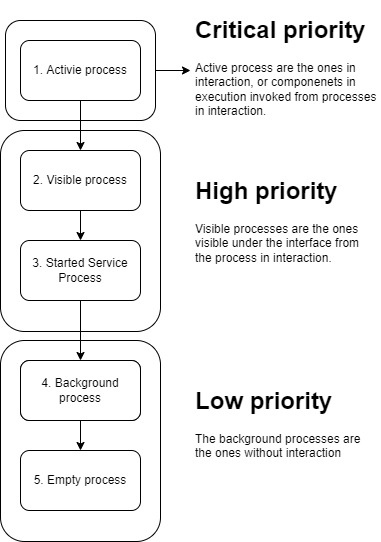
\includegraphics[width=0.4\linewidth]{figures/02_process_priority.png}
    \caption{Process priorities}
    \label{fig:process_priority}
    \end{figure}

% ACTIVITIES =======================================================================
\subsection{Activities}
    Usually show an user interface (using ViewGroups and Views) and inherit from android.app.Activity.
The activities execute a specific task in the application and the android always mantains a stack of 
activities. 

    Let's suppose that one activity inits another one. The first activity will go to the stack. When the 
back button is pressed, the first activity is retrieved from the stack. 

    An activity might be:
    \begin{itemize}
        \item active (runnning) - In interaction
        \item paused - Visible;
        \item Stopped - Non visible;
        \item Inactive (destroyed) - Without an instance object;
    \end{itemize}

    The android call lifecycle methods when there's a state transition.  



\subsubsection{In interaction vs Paused}
Let's suppose that we are running an active and then a dialog box pops up. Considering 
that the dialog box is managed by another activity, we can say that the previous activity is 
paused, but visible. The current activity (i.e the dialog box) is the active one. 

\subsubsection{Starting an activity}   
Before starting, take a look on the diagram below. This is the complete state diagram for android.

\begin{figure}[h]
    \centering
    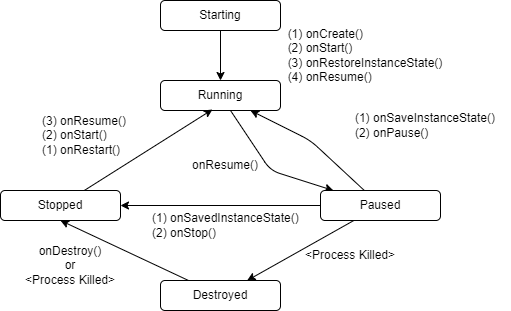
\includegraphics[width=0.8\linewidth]{figures/02_state_diagram.png}
    \caption{Activities State Diagram}
    \label{fig:state_diagram}
\end{figure}

Firstly the android system call life-cycle callbacks starting with the \textbf{onCreate()}. 

\begin{lstlisting}
// Always override
override fun onCreate(savedInstanceState: Bundle?){
    super.onCreate(savedInstanceState)
    val bt = findViewById<Button>(R.id.some_button)
    bt.setOnClickListener(this)
}
\end{lstlisting}

We should associate the listeners to interacion events in onCreate().


\subsubsection{Activity Navigation}
There are two criterias to the navigation:
\begin{itemize}
    \item Based on the past activated activity and the activity stack. This is usually 
    used when the user presses the \textbf{back button}.
    \item Based on a defined hierarchy. We can declare an activity parent in the manifest file 
    for each activity (except the one that starts the application); and a person can use the Up 
    button in the action bar to navigate.
\end{itemize}

% RESOURCES ========================================================================
\subsection{Resources}
The resources can be:
\begin{itemize}
    \item drawable - bitmaps, graphics, shapes, etc 
    \item anim - XML specifying animations between 2 configurations (tweens)
    \item color - colors (AARRGGBB) for many elements of the interface according to 
    state (pressed, focused, selected, ...)
    \item layout - screen organization 
    \item menu - options and context menus specifications 
    \item values - value collections with a name: string, arrays, colors, styles, dimensions,...
    \item xml - other XML files read with getXML()
\end{itemize}

\subsection{Events and listeners (IoC pattern)}

\subsubsection{Inversion of Control (IoC)}
IoC is the inversion control principle. Actually it's a principle, not a design pattern. 
This principle defines a basic characteristic of frameworks and it was popularized in 2004 by 
Robert C. Martin and Martin Fowler.  

Imagine that we have a code like this:

\begin{lstlisting}
public static void main(String[] args) {
    while (true) {
        BufferedReader userInputReader = new BufferedReader(
                new InputStreamReader(System.in));
        System.out.println("Please enter some text: ");
        try {
            System.out.println(userInputReader.readLine());
        } catch (IOException e) {
            e.printStackTrace();
        }
    }
}
\end{lstlisting}

The code is really simple: it will try to read the user input for undefined time and print in the console.
The main function/file has controls the program flow.  

Now consider that we've decided to use a GUI to do the same logic. The \textbf{framework is responsible for calling the user code.}
The framework is an extendable structure that provides the developer a set of specific points for injecting segments of the code.

\begin{tcolorbox}[title=IoC in short]
    In the case of frameworks that stick to the open/closed principle by 
    providing an extendable API, the role of the developer using the framework 
    boils down to defining their own set of custom classes, either by implementing 
    one or multiple interfaces provided by the framework or by inheriting from 
    existing base classes. In turn, instances of the classes are directly 
    instantiated from and called by the framework.
\end{tcolorbox}

\subsubsection{IoC in android}
In android the framework needs to listen the user code and execute it. Everytime a user makes an interaction, a message goes 
to a message queue, which is executed by a main thread (e.g UI thread). The main therad runs a 
loop that reads the message from the queue and makes a callback (life-cycle) or calls an event linstener (handler).

Here, the framework has the program flow. 


\subsection{Events generated by the interface}
Many views generate events, such as clicking in a button, changing focus, etc.  
We need to install listeners to these evets, by implementing the interfaces that describe them. 
Them implemented methods are called when the event occurs, such as:

\begin{itemize}
    \item onClick()
    \item onLongClick()
    \item onFocusChange()
    \item onKey()
    \item onTouch()
    \item onCreateContextMenu()
\end{itemize}

Defining a listerner is easy and can be defined in an activity: 

\begin{lstlisting}
// Listener defined in an activity
class ExampleActivity: Activity(), OnClickListener{
    ...
    val button = findViewById<Button>(R.id.corky);
    button.setOnClickListener(this);

}
// Implement the OnClickListener interface
override fun onClick(v: View){
    // Do something
}
\end{lstlisting}

As an anonymous object listener:
\begin{lstlisting}
override onCreate(savedValues: Bundle?){
    ...
    // Capture our button from layout
    val button = findViewById<Button>(R.id.corky)
    // Register the onClick listener with the implementation
    button.setOnClickListener(object: View.OnClickListener) {
        override fun onClick(v: View?){
            // do something
        }
    }
}
\end{lstlisting}
This last approach is no longer considered a good practivce, because it can create 
confusion and deeper dependencies between layouts and code. 

We can also use a lambda:

\begin{lstlisting}
    ... 
    button.setOnClickListener(v->btClick(v))
} 
fun btClick(v: View){
    // do something
}
\end{lstlisting}

\begin{tcolorbox}[colback=red!5,colframe=red!75!black, title=Disadvantages on IoC]
    A disadvantage of this pattern is that is one task takes too long, it will make the application slow.
    Because it's only one thread.
\end{tcolorbox}

% MENUS ============================================================================
\subsection{Menus}
There're two types of menu in android: the \textbf{option menus (associated to activities)} and the \textbf{context menu 
(associated to views)}. 


% TODO: not finished. 

\subsection{State preservation}

Standard activities in an application save some of their internal state whenever the activity is in
its way to the destroyed state. If the activity is active again it will restore its state before the
next time it is displayed.
This facility can be extended for non-standard activities (i.e., graphical) or other type of state.

Activities call onSaveInstanceState(Bundle) and onRestoreInstanceState(Bundle) when they need to
save and restore state (it is saved on memory).
These methods can be overridden in the derived class.

\begin{lstlisting}
override fun onSaveInstanceState(state: Bundle) {
    state.putFloat("Score", mCurrentScore)
    state.putInt("Level", mCurrentLevel)
    super.onSaveInstanceState(state)
    }
    override fun onRestoreInstanceState(state: Bundle) {
    super.onRestoreInstanceState(state)
    mCurrentScore = state.getFloat("Score")
    mCurrentLevel = state.getInt("Level")
    }
    
\end{lstlisting}

\subsection{Rotation}
When certain situation occurs that cause a change in device configurations
(rotating the devive, extending or hiding a logical keyboard, docking and undocking,
changing the locale or language), Android \textbf{destroys} and \textbf{re-creates} 
the running and paused activities, the next time are viewd. 

This could be necessary to load new resources for the user interface, more 
adapted to the new situation. 

Device rotation is a very common situation, and every user expects that all applications support
this change, eventually adapting the interface to portrait and landscape. 

When the activity is desstroyed, all internal variables loses their values, and 
the activity default mechanism default of saving state based on the \textbf{onSaveInstanceState()}
and \textbf{onRestoreInstanceState()} methods only saves and restores some of the internal
contents of the views (but not all).

Overriding this methods (e.g onRestoreInstanceState() and onSaveInstanceState()) 
we save information to the same bundle. But this bundle is saved in memory as long 
as the activity remains in the stack. If the process is popped from the stack (e.g 
click the back button) the Bundle is lost. 

\subsection{Feature and permissions}
Declared in the manifest when an application needs a certain hardware characteristic 
that can be unavailable. The features are defined in the Android class PackageManager. 

To use certain API functionalities the application needs permission from the user.
We can install it, by writing the permission in the manifest. 













    \section{Lecture 3 - Fragments}
    Activities were created to occupy the enterire screen and that's 
ok for small devices, but for large devices such as tablets,
we could use the space in a better way. 

Fragments can be seen as sub-activities, as they may respond to back-buttons 
and have their own \textbf{life-cycle}. However, a fragment lifecycle is 
related to the activity lifecycle. 
One activity can have many fragments and the point is that they all use the same 
thread (the main one).

\subsection{Fragment Lifecycles}

\begin{figure}[h]
\centering
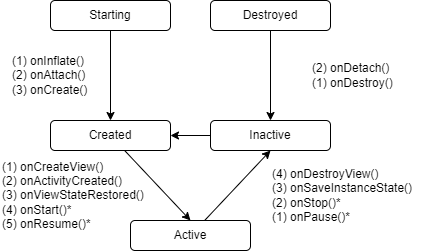
\includegraphics[width=0.8\linewidth]{figures/03_fragment_state_diagram.png}
\caption{Fragment State Diagram}
\label{fig:fragment_state_diagram}
\end{figure}


Now let's explain the sequence of commands called in a fragment life-cycle. 
\begin{itemize}
\item \texttt{onInflate(activity: Activity, attrs: AttributeSet, savedInstanceState: Bundle) }: Called in 
the beggining of the activity, when the fragment sets its content layout. The AttributeSet contains the attributes defined in the activity layout. They should be
parsed and saved. The fragment is not yet attached to the activity.

\item \texttt{onAttach(activity: Activity)}: Now the activity is attached to the fragment. In other words, 
it's possible to get the activity with the function \texttt{getActivity()} inside the fragment. 
It's also possible to get the arguments with \texttt{getArguments()}, but only the arguments set until
this moment.

\item \texttt{onCreate(savedInstanceState: Bundle)}: \textbf{It's when the fragment starts the process 
of creation} called at the beginning of the owner activity onCreate() callback. Usually, the 
\textbf{activity View hierarchy is not yet inflated}. You can create here another thread to do 
lengthy data loading operations.

\item \texttt{onCreateView(inflater: LayoutInflater, container: ViewGroup, savedInstanceState: Bundle)}:
This function should return the inflated View of this fragment. If the container is null, then null
must be returned. The container is the ViewGroup in the activity layout that will display the fragment.
Do not attach the fragment to this container. Some specialized fragments (e.g., ListFragment) do not need 
this callback.

\item \texttt{onActivityCreated(savedInstanceState: Bundle)}: here the onCreate() method of the activity 
is now complete. The complete interface is now built, including other present fragments. 

\item \texttt{onStart() and onResume()}: tied with the activity corresponding callbacks.

\item \texttt{onPause()}: the first to be called (the fragment can be put on the fragment back stack). You
should stop playing sounds, related to this fragment, here.

\item \texttt{onStop()} : tied with the onStop() callback of the activity. A stopped fragment can go straight
to the onStart() callback.

\item \texttt{onDestroyView()}: when the fragment is being killed or saved, this will be called. Here its View
hierarchy is already detached from the activity layout.

\item \texttt{onDestroy()}: is called when the fragment is no longer in use (but still existing in the activity).

\item \texttt{onDetach()}: here the fragment does not belong anymore to the activity and the interface
resources are already freed.

\item \texttt{onSaveIntanceState(outstate: Bundle)}: called somewhere before onDestroy(). It should save
internal state in the provided Bundle. That Bundle is passed to the entry callbacks.

\end{itemize}

\subsection{Fragment creation}

The fragment creation can be \textbf{STATIC} or \textbf{DYNAMIC}.

\begin{itemize}
    \item \textbf{STATIC}: Whenever the activity inflates its layout and has a <fragment> element in it, 
    the system constructs the Fragment
    \item \textbf{DYNAMIC}: If Fragments are built in the code, then a static factory method must be created in the fragment 
    class. It's recommended to have a factory for the fragment, since fragments doesn't have a constructor.
\end{itemize}

\begin{lstlisting}[title=Fragment Factory]
fun MyFragment newInstance(index: Int) {
    val f = MyFragment()
    val args = Bundle() 
    args.putInt("index", index)
    f.arguments = args
    return f
}
\end{lstlisting}

\begin{tcolorbox}[title=Bundled arguments]
    The arguments for a fragment inialization must be received in the factory must be passed as parameter
and then \textit{Bundled}. Bundled arguments are \textbf{preserved in the rotation} and are available as 
property.
\end{tcolorbox}

\subsection{Fragment Manager (supportFragmentManager)}
Activities and fragments can manager other active fragments. This can be done by using the 
\texttt{FragmentManager} object. This object is available at the property \texttt{supportFragmentManager}. 

It can:
\begin{itemize}
    \item Find fragments
    \item Manipulate the fragment back stack
    \item Save and restore references to fragments and fragment internal state
    \item Add, replace, remove, hiding and showing can be done and must be executed as a transaction.   
\end{itemize}

Example:

\begin{lstlisting}[title=Fragment transaction]
    /**
     * Changes the view to a fragment that shows the items inside the history.
     */
    private fun changeToBasketHistoryProducts(){
        val basketHistoryProducts = BasketHistoryProducts.newInstance(intent.extras!!)
        val fragmentManager = this.supportFragmentManager
        val fragmentTransaction = fragmentManager.beginTransaction()    // Starting transaction.
        fragmentTransaction.add(android.R.id.content, basketHistoryProducts)
        fragmentTransaction.commit()    // Should end with commit

    }
\end{lstlisting}

\subsection{Implementing a fragment}

\begin{lstlisting}[title=Fragment implementation]
    // In the parent activity
    class ParentActivity : AppCompatActivity() {  
      override fun onCreate(savedInstanceState: Bundle?) {  
        super.onCreate(savedInstanceState)  
        
        val frag = MyFragment.newInstance(intent.extras!!)  
        ... 
      }
      ...
    } 
     
    // In the Fragment class
    class MyFragment : Fragment() {
      var mIndex = 0;  
      
      override fun onCreate(savedInstanceState: Bundle?) {  
        super.onCreate(savedInstanceState)  
        mIndex = arguments?.getInt("index") ?: 0  
      }
        
      override fun onCreateView(inflater: LayoutInflater, container: ViewGroup?, savedInstanceState: Bundle?): View? {  
        if (container == null)  
          return null  
          
        // Don't tie this fragment to anything through the inflater
        val v = inflater.inflate(R.layout.details, container, false) 
        v.findViewById<TextView>(R.id.text1).text = Planets.PROPS[mIndex]  
        return v  
      }  
      
      // Fragment factory
      companion object {  
        @JvmStatic
        fun MyFragment newInstance(index: Int) { 
          val f = MyFragment() 
          val args = Bundle()
          args.putInt("index", index) 
          f.arguments = args 
          return f 
        }
      }
    }
    
\end{lstlisting}

\textbf{NOTE}: The method of building dialogs from the Dialog class doesn't take care 
automatically of lifecycle events, like the destruction and re-creation. You should embed the 
\texttt{DialogFragment}. 




    \section{Lecture 4 - NFC}
    There're three modes that the NFC can work:

\begin{itemize}
    \item Read and write tags (good, API 10);
    \item Peer-to-Peer (beam/limited, API 14);
    \item Card emulator (real/emulated SE, API 19); 
\end{itemize}


The android hardware can include a \textbf{secure element} which is similar to a smartcard running 
JavaCardOS. For more information about JavaCardOS you can read:

https://www.oracle.com/java/technologies/java-card/javacard1.html

\subsection{NdefMessage class} 
Android supports NFC messages by using \texttt{NdefMessage} class.

\begin{lstlisting}[title=Using NdefMessage class]
val mimeType = "application/my.mime.type" // a custom mime type
val payload = "This is a TNF_MIME_MEDIA"
val mimeRecord = NdefRecord.createMime(mimeType, payload.getBytes(Charsets.UTF_8))
val newMessage = NdefMessage(arrayOf(mimeRecord))
\end{lstlisting}

The constructor \texttt{NdefMessage} accepts a list of records 
(\texttt{NdefRecord}) and these methods can be obtained through 
\texttt{getRecords()} method. 

The \texttt{NdefRecord} constructor is: \texttt{NdefRecord(tnf: Short, 
type: ByteArray, id: ByteArray, payload: ByteArray)}. 

The type, id and payload are conditioned by the TNF field. 

\begin{itemize}
    \item \textbf{Tags}:  TNF values of TNF\_ABSOLUTE\_URI or TNF\_WELL\_KNOWN 
    are usually used, with corresponding values of type, id, and payload. 
    \item \textbf{Device to device messaging}:  the TNF value is usually 
    TNF\_MIME\_MEDIA with a custom media type in type, an id of 0 bytes, 
    and a payload.
\end{itemize}

The \texttt{NdefRecord} class has get methods for the TNF, type, id, and payload constituents.
It has also static \texttt{NdefRecord} methods for building some kinds of records, like
\texttt{createMime()}.

\subsection{Setup manifest}

The following code must be added:
\begin{lstlisting}
    <uses-permission android:name="android.permission.NFC" />
    <uses-sdk android:minSdkVersion="10"/>
    <uses-feature android:name="android.hardware.nfc" android:required="true" />
\end{lstlisting}

Not finished.......................................................AAAAAAHHH!





    \newpage
    \section{Lecture 5 - Android HTTP and Asynchronous processing}
    \subsection{HTTP request}
Calling webservices uses HTTP protocols. 

To execute this, \textbf{a separate thread is necessary} as well as a manifest permission:

\begin{lstlisting}
<uses-permission android:name="android.permission.INTERNET"/>
\end{lstlisting}

After API 27, only HTTPS is allowed by default. Use \texttt{android:usesCleartextTraffic="true"}  in the 
\texttt{<}application\texttt{>} manifest tag for allowing HTTP. 

\begin{lstlisting}[title=Using HttpURLConnection]
private class AddUser(val address: String, val uname: String) : Runnable {
    override run() {
        val url: URL? = null
        val urlConnection: HttpURLConnection? = null
        try {
        // Configure -------------------------------------------
        url = URL("http://" + address + ":8701/Rest/users")
        urlConnection = url.openConnection() as HttpURLConnection
        urlConnection!!.setDoOutput(true)
        urlConnection!!.setDoInput(true)
        urlConnection!!.setRequestMethod("POST")
        urlConnection.!!setRequestProperty("Content-Type", "application/json")
        urlConnection!!.setUseCaches(false)

        // Payload ---------------------------------------------
        val outputStream = DataOutputStream(urlConnection!!.getOutputStream())
        val payload = "\"" + uname + "\""
        outputStream.writeBytes(payload)
        outputStream.flush()
        outputStream.close()

        // Response --------------------------------------------
        val responseCode = urlConnection!!.getResponseCode()
        if (responseCode == 200)
        val response = readStream(urlConnection!!.getInputStream(); // ... and transmit to UI
        }
        catch (Exception e) { . . . // treat the exception
        }
        finally {
            if(urlConnection != null) urlConnection.disconnect()
        }
    }
}
\end{lstlisting}

\begin{lstlisting}[title=Using threads to invoke]
val addUser = AddUser(address, name)
val thr = Thread(addUser)
thr.start();
\end{lstlisting}

\subsection{Threads}
When an application is launched, the system creates a thread of execution for the 
application, called "main." This thread is in charge of dispatching events to the 
appropriate user interface widgets and for interacting with components from the Android UI 
toolkit. As such, the main thread is also sometimes called the UI thread. 


Android UI toolkit is not thread-safe. So, you must not manipulate your UI from a 
worker thread—you must do all manipulation to your user interface from the UI thread. 
Activity.runOnUiThread(Runnable) is a way to access the UI thread from another thread to 
solve this problem.

\subsection{Communication between threads}
The problem with the java communication systems between threads (e.g pipes, blocking queue, 
shared memory, etc) is that these mechanisms are blocking. Since the communication between threads
are mainly done between the UI thread and background threads, an android mechanism was created to handle
this communication. 

\subsubsection{Handlers}

\begin{figure}[h]
\centering
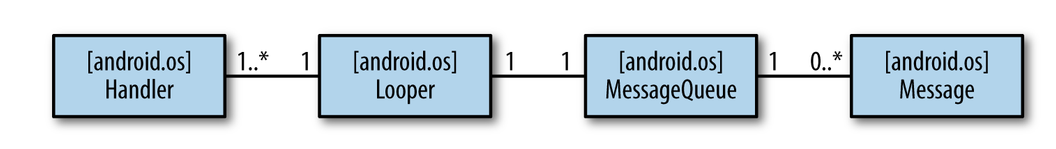
\includegraphics[width=0.8\linewidth]{figures/05_thread_handler_overview.png}
\caption{Thread handler overview}
\label{fig:thread_handler_overview}
\end{figure}

\begin{itemize}
    \item \texttt{android.os.Looper}: A message dispacher associated with one and only 
    one cosumer thread. 
    \item \texttt{android.os.Handler}: Consumer thread message processor, and 
    the interface for a producer thread to insert messages into the queue.
    A Looper can have many associated handlers, but they \textbf{all insert messages into 
    the same queue}.
    \item \texttt{android.os.MessageQueue}: Unbounded linked list of messages to be processed 
    on the consumer thread. Every Looper - and Thread - has at most one MessageQueue.
    \item \texttt{android.os.Message}: Message to be executed on the consumer thread.
\end{itemize}



\begin{lstlisting}[title=Send messages between threads]
// Cosumer threads 
MyHandler(val uiActivity: MyActivity) { 
    override handleMessage(m: Message) { 
        val s = m.getData().getString("msgstr") 
        // ... uiActivity.doSomething(s) 
    } 
}

// Producer threads
MyRunnable(val uiHandler: Handler) { 
    fun run() { 
        ...interact()...
    } 
    fun interact() { 
        val m = uiHandler.obtainMessage() 
        m.setData(createBundleFromStr("something")) 
        // boolean sendMessage(Message msg)
        uiHandler.sendMessage(m) // Send message to the queue. 
    } 
}
    
// In the activity
val myHandler = MyHandler(this)
val worker = Thread(MyRunnable(myHandler))
worker.start()
    
\end{lstlisting}

The code above follows the schema:
\begin{figure}[h]
\centering
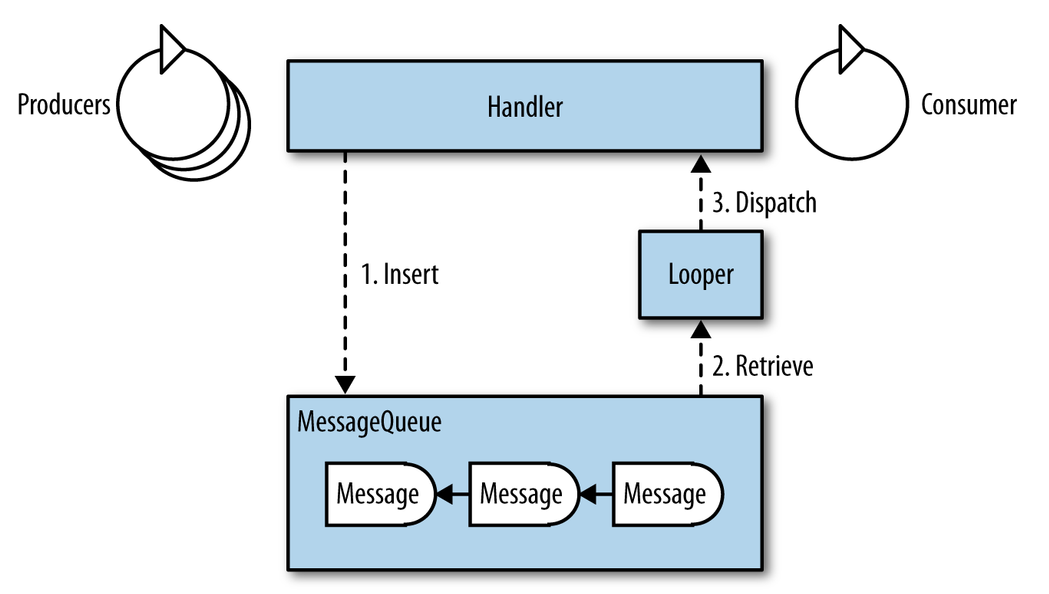
\includegraphics[width=0.8\linewidth]{figures/05_handler_schema.png}
\caption{Sending message flow schema}
\label{fig:handler_schema}
\end{figure}


\newpage
\subsubsection{Messages as Tasks (Post)}
The Handler inserts messages in the message queue in various ways depending on the 
message type. 
\begin{itemize}
    \item Task messages are inserted through methods that are prefixed post;
    \item Data insertion methods are prefixed send, like we saw in the previous section. 
\end{itemize}

To add a task in a queue we can do:
\begin{lstlisting}
boolean post(Runnable r)
\end{lstlisting}


\begin{lstlisting}[title=Post an no parameters]
private val handler = Handler()

private fun mainProcessing() { 
    val thread = Thread(doBackgroundThreadProcessing, "Background") 
    thread.start() 
} 
    
private val doBackgroundThreadProcessing = Runnable() {
    override run() { 
        [ ... Time consuming operations ... ]
        handler.post(doUpdateGUI) // send a task to the queue. 
    } 
}
    
// Runnable that updates GUI on the UI thread
val doUpdateGUI = Runnable() { 
    override run() { 
        [ ... Open a dialog or modify a GUI element ... ] 
    } 
};

\end{lstlisting}
\newpage
\subsection{Async Task}
The message passing mechanism between thread is a \textbf{nonblocking} consumer-producer pattern. 
\begin{lstlisting}[title=Creating and running Async tasks]
// AsyncTask<[Input Parameter Type], [Progress Report Type], [Result Type]>
private class MyAsyncTask() : AsyncTask<String, Int, Int> {
    // Is also executed by the UI thread when the background task call publishProgress.
    There is parameter passing between these methods. 
    override onProgressUpdate(progress: Int) {
        // [... Update progress bar, Notification, or another UI element ...]
    }

    // Is executed by the UI Thread when doInBackground finishes. 
    override onPostExecute(result: Int) {
        // [... Report results via UI update, Dialog, or notification ...]
    }

    // Is executed by a background task when AsyncTask is excuted.
    override doInBackground(parameter: String ): Int {
        val myProgress = 0
        // [... Perform background processing task, update myProgress...]
        publishProgress(myProgress)
        // [... Continue performing background processing task ...]
        // Return the value to be passed to onPostExecute
        return result
    }
}

// Executing 
MyAsyncTask().execute("inputString");
    
\end{lstlisting}












    \section{Lecture 6 - Broadcast, Services and Notifications}
    \subsection{Broadcast}
\hl{Are application components that can receive 'intents' from other 
components.}

\hl{We can use the broadcast to send information to another app and inside the same app.}

Broadcast receivers can be declared in \textbf{the manifest} or 
\textbf{registered dynamically}. 

They also can have an associated ACTION or cross-application explicit 
intent. 

Are invoked using \texttt{sendBroadcast()}, which can be invoked by
any other component or other application. 

To receive the broadcast message, one must use the \texttt{BroadcastReceiver}. 
It's necessary to override the \texttt{onReceive} class, because this class
doesn't have any user interface. 

Let's create a \texttt{BroadcastReceiver} and declare it in the manifest:

\begin{lstlisting}
...
<application>
...
<receiver android:name=" ... " >
<intent-filter>
<action android:name=" ... " />
</intent-filter>
</receiver>
...
\end{lstlisting}

In the activity, we gonna send the a broadcast message:

\begin{lstlisting}
Intent bi = ... // should match the name of the action in the manifest. 
sendBroadcast(bi);
\end{lstlisting}

An example is: 
\begin{lstlisting}[title=Manifest definition]
<manifest>
    <application>
        ...
        <receiver android:name=".MyReceiver">
            <intent-filter>
                <action android:name="org.feup.intents.test" />
            </intent-filter>
        </receiver>
        ...
    </application>
    ...
</manifest>
\end{lstlisting}

\begin{lstlisting}[title=Broadcast activity]
public class MyActivity extends Activity {
    ...
    private void invokeReceiver() {
        Intent broadcast = new Intent ( "org.feup.intents.test");
        broadcast.putExtra("somename", "Hello");
        sendBroadcast(broadcast);
    }
    ...
}
\end{lstlisting}

\begin{lstlisting}[title=The receiver]
// This class can be instatiated in any component. 
public class MyReceiver extends BroadcastReceiver {
    @Override
    public void onReceive(Context context, Intent intent) {
        String msg = intent.getStringExtra("somename");
        //Do something
    }
}
\end{lstlisting}

\subsection{Services}

\hl{As we have seen before the services are invisible to the user and are not an
asynchronous execution itself.} The \textbf{Service runs in the UI thread}, so it 
can degrade responsiveness and cause ANRs (application not responding), even 
though it does not interact directly with the UI. Still, the \texttt{Service} in 
combination with asynchronous executor is a powerful tool for background task 
execution. 

\subsubsection{Why use a Service for asynchronous execution?}

\begin{itemize}
    \item \textit{Decouple lifecycles of components and threads}: Even after 
    the component that started the thread finishes itself, the thread will continue 
    running. Threads may keep references to Java objects so that they cannot be 
    garbage collected until the thread terminates. 
    \item \textit{Lifecycles of the hosting process}: If the runtime terminates the 
    process, all of its threads are terminated and not restarted by default when the 
    process is restored. A process with no active components is likely yo be eligible 
    for termination, since a task with no components contains low rank. For example, 
    an \texttt{Activity} stores user data to a database in a background thread
    while the user navigates back leaves an empty process if there are no other 
    components running. This increases the risk of process termination, aborting the 
    background thread before it can persist the data. 
\end{itemize}

\hl{Thus, a \texttt{Service} can mitigate both the risk for memory leaks and the risk of 
having tasks terminated prematurely. \textbf{Services has high priority}, but still 
less, than activities.}

\subsubsection{Creation and Execution}

\begin{lstlisting}
    public class EatService extends Service {
        @Override
        public void onCreate() { /* Initialize component */ }
        
        @Override 
        public void onDestroy() {/* Clean up used resources*/} 

        @Override
        public IBinder onBind(Intent intent) { /* Return communication interface */ } 
    }
\end{lstlisting}

The only mandatory method is \texttt{onBind}, which returns the communication 
interface to the client to perform remote call services. 

To \textbf{start} the service, one can call \texttt{startService(Intent)} and to stop 
it's possible to call \texttt{stopService(Intent)} or \texttt{Service.stopSelf()}. 


\begin{figure}[h]
\centering
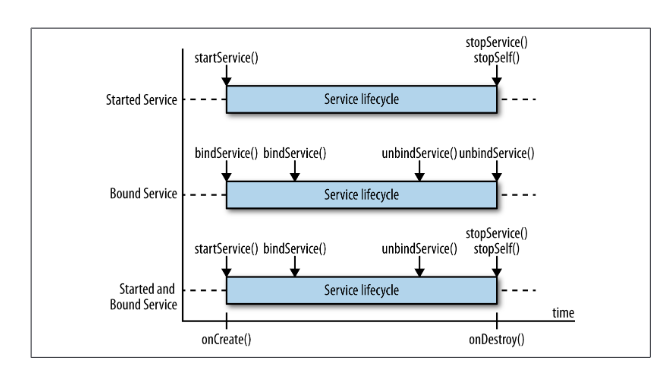
\includegraphics[width=1\linewidth]{figures/06_service_lifecycle.png}
\caption{Service lifecycle}
\label{fig:service_lifecycle}
\end{figure}

\subsubsection{Started service}
Components invoke Context.startService(Intent) to send start requests to a \texttt{Service},
which can be invoked by multiple components and multiple times from every components during 
lifecycle. The first start request creates and starts the \texttt{Service}, whereas consecutive
start requests just pass on the \texttt{Intent} to the started \texttt{Service} so that the
data conveyed in the \texttt{Intent} can be processed. 

Services always have to implement onBind, but started services—which do not support
binding—should provide a trivial implementation that just return null:

\begin{lstlisting}
public class StartedEatService extends Service {
    @Override
    public int onStartCommand(Intent intent, int flags, int startId) { ... }

    @Override
    public IBinder onBind(Intent intent) { return null; }
}
\end{lstlisting}

Started services must implement an \texttt{onStartCommand} method that handles start
requests. The method is invoked each time a start request (\texttt{Context.startService})
from a client component is ready to be processed. 

Start requests are delivered sequentially to onStartCommand and remain pending in 
the runtime until preceding start requests are processed or offloaded from the UI thread.

\begin{tcolorbox}[colback=red!5,colframe=red!75!black, title=Problems of onStartCommand]
onStartCommand is executed on the UI thread, so you should spawn background threads
within the method to execute long-running operations, not only to preserve responsiveness 
but also to enable concurrent execution of multiple start requests.

\end{tcolorbox}

\texttt{onStartCommand} is the key method for implementing started Services and intiating
asynchronous task execution. The arguments are: 

\begin{itemize}
    \item \textit{Intent}: Data to be used for the asynchronous execution; e.g., a URL to a network resource
    that shall be retrieved. 
    \item \textit{Delivery method}: A flag reflecting the history of the start request. 
    This argument may contain other flags in future versions of Android. 
    Possible values are currently 0, START\_FLAG\_REDELIVERY (value of 1), or 
    START\_FLAG\_RETRY (value of 2). 
    \item \textit{StartID}: A unique identifier provided by the runtime for this start request. If the process is
terminated and restarted, onStartCommand is called with the same start ID.
\end{itemize}

The return value of \texttt{onStartCommand} and the second argument (the delivery method flag)
let you control what happens after your \texttt{Service} is terminated. It tells the runtime 
weather to restart the \texttt{Service} and resubmit the \texttt{Intent} argument, in case 
the runtime has to terminate the process for lack of resources and then restart it.

\subsubsection{Options for restarting} 
ike any Android application, your Service may be terminated by the runtime if there 
are too many processes running on the device. In fact, as a background process, your 
Service has a greater chance of being killed than many other processes.

This section covers termination by either the runtime or a client, not a clean termination 
through \texttt{Service.stopSelf}.

The values that the \texttt{onStartCommand} may return are: 
\begin{itemize}
    \item \texttt{START\_STICK}: The \texttt{Service} will be restarted in a new process whether
    or not here are any requests pending. The resources are brought to memory again, but with a 
    \texttt{NULL} intent, because \texttt{onStartCommand} is invoked with a \texttt{null} value for 
    the \texttt{Intent} argument. However, the \texttt{Service} will receive any pending start requests
    that remained undelivered when the previous \texttt{Service} process was terminated. The pending 
    start requests are delivered with the \texttt{START\_FLAG\_RETRY} set in the call's second argument. 

    \item \texttt{START\_NOT\_STICK}: Like \texttt{START\_STICK}, except that the \texttt{Service} will be 
    restarted only if there were pendind start requests when the process was terminated. An \texttt{Intent} will
    always be passed. Then the resources are not brought back to memory until a new \texttt{startService} is
    executed.
    \item \texttt{START\_REDELIVER\_INTENT}: The \texttt{Service} will be restarted and reves both pendind requests
    and requests that were previously started and had no change to finish. The pending requests are 
    delivered with the \texttt{START\_FLAG\_RETRY} set in the second argument, whereas the previously 
    started requests are redelivered with the \texttt{START\_FLAG\_REDELIVERY} set. The resources are 
    brought to memory again with the last process intent. 
\end{itemize}

\subsubsection{Example}

\begin{lstlisting}[title=Service code template]
import android.app.Service;
import android.content.Intent;
import android.os.IBinder;
public class MyService extends Service {
    @Override
    public void onCreate() {
        // TODO: Actions to perform when service is created.
    }
    @Override
    public IBinder onBind(Intent intent) {
        return null; // mandatory but should return null for
        // non remote call services
    }
    @Override
    public int onStartCommand(Intent intent, int flags, int startId) {
        // Usually launch a background thread to do processing.
        return Service.START_NOT_STICKY; // or other value
    }
    @Override
    public void onDestroy() {
        // TODO: Actions to perform when service is destroyed
    }
}
\end{lstlisting}

\begin{lstlisting}[title=Manifest]
    <service android:name=".MyService"/>
\end{lstlisting}

\begin{lstlisting}[title=Calling the service]
// Implicitly start a Service
Intent myIntent = new Intent(MyService.ORDER_PIZZA);
myIntent.putExtra("TOPPING", "Margherita");
startService(myIntent);

// Explicitly start a Service in the same process
startService(new Intent(this, MyService.class));
\end{lstlisting}

\begin{lstlisting}[title=Stoping the service]
// With the same intent
stopService(new Intent(MyService.ORDER_PIZZA));

// Stop a service with the service name (same proc).
ComponentName service = startService(new Intent(this, MyService.class));
...
stopService(new Intent(this, service.getClass()));

// Stop a service explicitly in the same process
Class serviceClass = Class.forName(service.getClassName());
stopService(new Intent(this, serviceClass));
\end{lstlisting}


\subsection{Intent service}
It's a special purpose Service subclass that creates a single worker thread.
The intent received on \texttt{onStartCommand()} is passed to the method that 
the worker thread executes.

The \texttt{IntentService} is suitable for when you want to offload tasks easily 
from the \texttt{UI thread} to a background thread with sequential task processing, 
giving the task a component that is always active in order to raise the process rank.

Successive calls on \texttt{onStartCommand()} are queued. You only have to override and implement
\texttt{onHandleIntent()}. 

\begin{lstlisting}[title=IntentService implementation]
public class MyService extends IntentService {
    public MyService() {
        super("MyService");
    }
    @Override
    protected void onHandleIntent(Intent intent) {
        // Do the work in this single worker thread
        // and return
    }
}
\end{lstlisting}

\subsection{Result Service}
Mechanism to return a result to an \texttt{Activity} (or other component activated by an \texttt{Intent}) from
other component or thread (using a \texttt{Handler()}). 

It is created on the destination with \texttt{onReceiveResult()} overridden.
As this class is \texttt{Parcelable} their objects can be passed in Intent.
The recipient sends results using \texttt{send()}, triggering a call to \texttt{onReceiveResult()}.

\subsubsection{Example}

\begin{lstlisting}[title=Recipient component (an activity)]
//recipient Activity
public class MainActivity extends AppCompatActivity {
    // some variables (Activity state)
    ....
    @Override
    protected void onCreate(Bundle savedInstanceState) {
        ...
        Intent aService = new Intent(this, MyService.class);
        aService.putExtra(MyService.RESULT, new ResultReceiver(new Handler()) {
            @Override
            protected void onReceiveResult(int code, Bundle data) {
                super.OnReceiveResult(code, data);
                .... // if code OK, use data and other Activity state
                ....
            }
        });
    }
}
\end{lstlisting}

\begin{lstlisting}[title=A service sending results]
public class MyService extends Service {
    public final static String RESULT = "RemoteResult";
        ...
    @Override
    public int onStartCommand(Intent i, int flags, int sId) {
        ResultReceiver rec = i.getParcelableExtra(MyService.RESULT);
        ...
        Bundle data = new Bundle();
        data.putString("value", "some data");
        ...
        rec.send(1, data);
        return Service.START_NOT_STICKY;
    }
    ...
}
\end{lstlisting}


\subsection{Remote Call Services (RPC)}

Their functionality is invoked using RPC. Usually, they are standalone in their own processes. 

Remote call services are activated (brought to memory and \texttt{onCreate()} invoked) through
\texttt{bindService()} and can be freed when the last bound client calls \texttt{unbindService()}.

When a service is ready to be called through its interface a callback  \texttt{onServiceConnected()} is 
called on the client.

There is also a \texttt{onServiceDisconnected()} callback on the client that is called when the 
service is not available (motivated by a crash or reclaimed by Android). 

\begin{figure}[h]
\centering
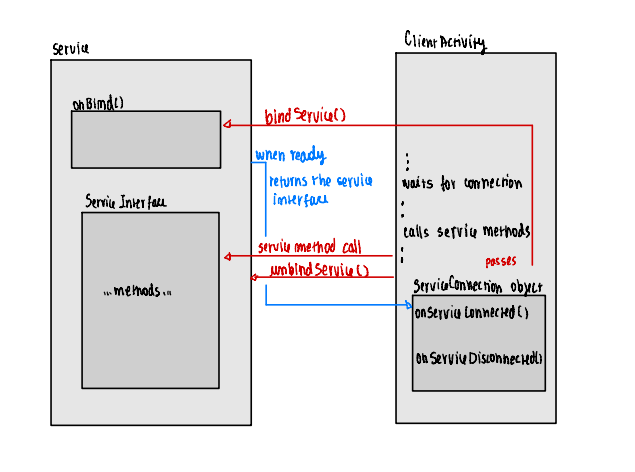
\includegraphics[width=1\linewidth]{figures/06_RPC_flow.png}
\caption{RPC flow}
\label{fig:rpc_flow}
\end{figure}

\subsubsection{Example}

\begin{lstlisting}[title=Service interface is defined in the AIDL file]
// This file is IStockQuoteService.aidl
package com.androidbook.services.stockquoteservice;
    interface IStockQuoteService {
    double getQuote(String ticker);
}
\end{lstlisting}

\begin{lstlisting}[title=Service must implement the interface]
public class StockQuoteService extends Service {
    public class StockQuoteServiceImpl extends IStockQuoteService.Stub {
        @Override
        public double getQuote(String ticker)
            throws RemoteException {
                return 20.0;
            }
        }
    @Override
    public IBinder onBind(Intent intent) {
        return new StockQuoteServiceImpl();
    }
}

\end{lstlisting}

\begin{lstlisting}[title=Client calling the service]
...
bindService(new Intent(IStockQuoteService.class.getName()), serConn, Context.BIND_AUTO_CREATE);
...
private ServiceConnection serConn = new ServiceConnection() {
    @Override
    public void onServiceConnected(ComponentName name, IBinder service) {
        stockService = IStockQuoteService.Stub.asInterface(service);
        callBtn.setEnabled(true);
    }

    @Override
    public void onServiceDisconnected(ComponentName name) {
        callBtn.setEnabled(false);
        stockService = null;
    }
};
...
try {
    double val = stockService.getQuote("ANDROID");
    Toast.makeText(this, "Value from service is " + val, Toast.LENGTH_SHORT) .show();
} catch (RemoteException ee) {
}
\end{lstlisting}

\subsection{Notifications}
Are shown in the status bar. More details listed in the extended status drawer. 
They can produce sound, vibration and light leds. 

They are created using a system service:
\begin{lstlisting}[title=Creating notifications]
String svcName = Context.NOTIFICATION_SERVICE;
NotificationManager notificationManager;
notificationManager = (NotificationManager) getSystemService(svcName);
\end{lstlisting}

Are specified in a Notification object through a Build class:
\begin{lstlisting}[title=Build class]
// A small icon, a title and a text and mandatory (many other features)
// get the Notification object using the build() method
Notification notf = new Notification.Builder(this)
.setContentText(message) // the main text of the notification
.setContentTitle(title) // the first line (title)
.setSmallIcon(R.drawable.nticon) // icon on bar and notification
.setWhen(System.currentTimeMillis()) // for ordering
.setPendingIntent(PendingIntent pi) // Activity to launch on tap
.build(); // returns the notification object
notf.flags |= Notification.FLAG_ONGOING_EVENT; // cannot be cleared
\end{lstlisting}

Sent using the \texttt{notify()} method of the service.

Notifications are customizable. 

\subsection{Alarms}

Calls an application component periodically or after a specified time interval and uses another 
system service: 
\begin{lstlisting}[title=Creating an alarm]
String svcName = Context.ALARM_SERVICE;
AlarmManager alarms;
alarms = (AlarmManager) getSystemService(svcName);
\end{lstlisting}

We can use the methods \texttt{set()}, \texttt{setRepeating()} or \texttt{setInexactRepeating()} to create alarms. 

\begin{lstlisting}
int alarmType = AlarmManager.ELAPSED_REALTIME_WAKEUP;
long timeOrLengthOfWait = 10000;
String ALARM_ACTION = "ALARM_ACTION";
Intent intentToFire = new Intent(ALARM_ACTION);
PendingIntent pendingIntent = PendingIntent.getBroadcast(this, 0, intentToFire, 0);
alarms.set(alarmType, timeOrLengthOfWait, pendingIntent);
\end{lstlisting}









    \section{Lecture 7 - Sensors}
    \subsection{Location Providers}

A device may have several providers. Location can be obtained directly from satellites 
(GPS). Or can be derived from Wi-fi access points information, mobile communication tower's location. 

The devices are condensed in the provider: GPS\_PROVIDER ("gps"), NETWORK\_PROVIDER ("network").
Also usually exists a PASSIVE\_PROVIDER (another app) 

GPS is accurate, has more info, more power consumption, more delay,
needs line of sight to satellites (weak signals). 

Network is less accurate, has less consumption, less delay, interiors.

Android manifest must declare permissions:

\begin{itemize}
    \item ACCESS\_COURSE\_LOCATION
    \item ACCESS\_FINE\_LOCATION
\end{itemize}

\begin{figure}[h]
\centering
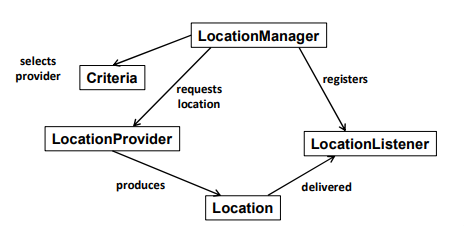
\includegraphics[width=0.9\linewidth]{figures/07_location_manager_diagram.png}
\caption{Location Manager Diagram}
\label{fig:location_manager_diagram}
\end{figure}


\subsection{LocationListener} 
Interface declaring methods (callbacks) where information is delivered
after requesting a location. 

\begin{lstlisting}[title=LocationListener interface]
public interface LocationListener {
    void onLocationChanged(Location location);
    void onProviderDisabled(String provider);
    void onProviderEnabled(String provider);
    // Not called in api 29.
    // status: OUT_OF_SERVICE, TEMPORARILY_UNAVAILABLE,AVAILABLE
    // satelities: nr. of satelities in gps. 
    void onStatusChanged(String provider, int status, Bundle extras);
}
\end{lstlisting}

\subsection{LocationManager}

System service for requesting locations and selecting a provider. 
Obtained in an Activity: 

\begin{lstlisting}
locationManager = (LocationManager) getSystemService(LOCATION_SERVICE);
\end{lstlisting}

Locations should be requested only when the activity is active and cancelled 
when it stops being in foreground.
So requests can be done in the \texttt{onResume()} callbackof the activity, 
from the LocationManager object, with:

\begin{lstlisting}
// minTime: minimum time or distance for a new location
// criteria: selection of a provider 
// listener: class implementing the listener
// looper: null for the current thread
requestLocationUpdates(long minTime, float minDistance, Criteria criteria,LocationListener listener, Looper looper); 
\end{lstlisting}

In \texttt{onPause()} we should cancel the request and stop the provider:

\begin{lstlisting}
removeUpdates(LocationListener listener) 
\end{lstlisting}


It is also possible to request a single location or an alert of proximity to agiven location expressed in latitude or longitude.
\texttt{requestSingleUpdate(...) and addProximityAlert(...)}. 

\subsection{Location}
Locations are delivered to LocationListener 

\begin{itemize}
    \item They bring latitude and longitude;
    \item The provider that has generated it;
    \item The time it was generated;

\end{itemize} 

If the provider have the information, it can also contain: 
\begin{itemize}
    \item The altitude of the location;
    \item The accuracy of the location;  
    \item The bearing if the device is moving
    \item The speed also if it is moving
    \item The number of satellites used to obtain the location
\end{itemize} 

Some convenience methods allow: 
\begin{itemize}
    \item To know the bearing from this location to another (geodesic)
    \item The distance between locations (along a geodesic)
    \item Obtain a convenient String representation
\end{itemize}

\begin{figure}[h]
\centering
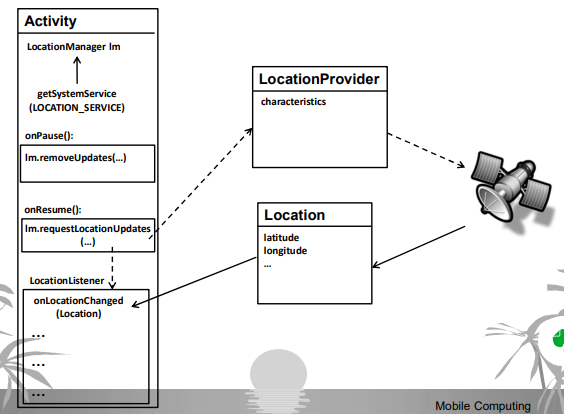
\includegraphics[width=0.8\linewidth]{figures/07_receiving_location_information.png}
\caption{Receiving location information}
\label{fig:receiving_location_information}
\end{figure}

\subsection{Sensors}
Android has support for several sensors and a common API to get their measurements.
Sensors available include:
\begin{itemize}
    \item  movement sensors; 
    \item  orientation sensors;
    \item  environment sensors;
\end{itemize} 

Sensors can be divided into: 
\begin{itemize}
    \item physical sensors giving actual measurements of some quantity;
    \item synthesized sensors fusing and processing the measurements of other physical sensors to calculate another quantity;
\end{itemize}

Sensors can be characterized by:
\begin{itemize}
    \item Range and resolution (minimum, maximum and step value);
    \item Rate of measurement (nr. of measurements per time unit);
    \item Power consumption;
\end{itemize}

\subsubsection{Sensor type supported}

Android defines a constant for each of the 
sensor types supported bythe operating system, in the Sensor class. 
But each device may haveonly a few of those sensors.

\begin{lstlisting}[title=physical types]
movement:
    TYPE_ACCELEROMETER (3D)
    TYPE_GYROSCOPE (3D)
orientation:
    TYPE_MAGNETIC_FIELD (3D)
environment:
    TYPE_AMBIENT_TEMPERATURE
    TYPE_LIGHT
    TYPE_PRESSURE
    TYPE_PROXIMITY
    TYPE_RELATIVE_HUMIDITY
\end{lstlisting} 

\begin{lstlisting}[title=synthetized types]
TYPE_GRAVITY (3D)
TYPE_LINEAR_ACCELERATION (3D)
TYPE_ORIENTATION (3D)
TYPE_ROTATION_VECTOR (3 or 4D)
TYPE_SIGNIFICANT_MOTION (Trigger)
\end{lstlisting}

\subsubsection{Sensor on a device}
It's possible for a device to have more than one sensor of the same type.
It's uncommon for physical sensors, but can happen with synthesized
sensors (more than one implementation). 

When an application requests the sensors
of a certain type (with \texttt{getSensorList(type)}),
the system returns an array of sensors. 


The \texttt{SensorManager} is the starting point and can be obtained from
the \texttt{Activity} with:

\begin{figure}[h]
\centering
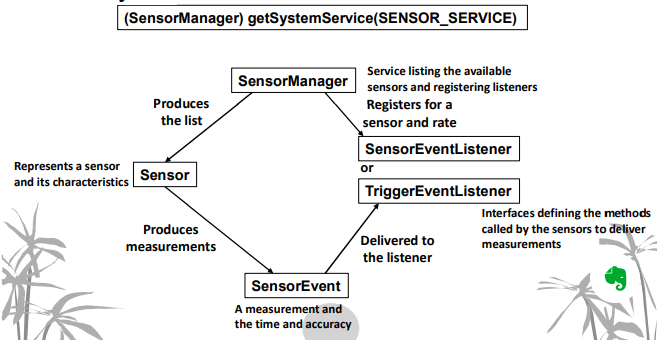
\includegraphics[width=0.8\linewidth]{figures/07_sensor_api_classes.png}
\caption{Sensor API classes}
\label{fig:sensor_api_classes}
\end{figure}

\subsubsection{Movement and Orientation}
Movement quantities are presented in the device coordinate system.
Orientation measures are in the earth coordinate system (except
\texttt{TYPE\_ORIENTATION} and \texttt{getOrientation()} measurements).

\texttt{TYPE\_ORIENTATION} and \texttt{getOrientation()} measurements earth coordinate system.

\begin{figure}[h]
\centering
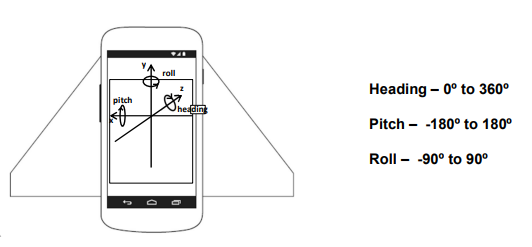
\includegraphics[width=0.8\linewidth]{figures/07_orientation_measurements.png}
\caption{Orientation measurements}
\label{fig:orientation_measurements}
\end{figure}

\subsubsection{SensorManager}

Activities get it from the system and it knows the sensors available on the device.
We can get a list of all or of a single type of sensors and it's possible to have more than one sensor of a given type
(specially of fusion/synthesized sensors). 

It can register the \texttt{SensorEventListener} for one or
more sensors. 
It defines some measure transformation methods: 
\begin{itemize}
    \item \texttt{getRotationMatrixFromVector()} uses the \texttt{ROTATION\_VECTOR} 
sensor and computes a rotation matrix;
    \item \texttt{getRotationMatrix()}: computes Inclination and Rotation matrices from gravity and
geomagnetic fields
\item \texttt{getInclination()} (from the Inclination matrix)
\item \texttt{getOrientation()} (from the Rotation matrix)
\item \texttt{getAltitude()}  From the atmospheric pressure here and at sea level

\end{itemize}

\subsubsection{SensorEventListener}
Interface declaring methods (callbacks) where measurements are
delivered after registering it for a sensor.
Measurements are represented by an instance of \texttt{SensorEvent}. 

\begin{lstlisting}
public interface SensorEventListener {
    // The event has sensor, values[], timestamp, accuracy
    void onSensorChanged(SensorEvent event);
    void onAccuracyChanged(Sensor sensor, int accuracy);
}

// The accuracy can be one of SENSOR_STATUS_ACCURACY_HIGH, SENSOR_STATUS_ACCURARY_MEDIUM,
// SENSOR_STATUS_ACCURACY_LOW, SENSOR_STATUS_ACCURARY_UNRELIABLE. 

// For sensors producing an event at a time (like the SIGNIFICANT_MOTION detector)
// use the abstract class:
public abstract class TriggerEventListener {
    public void onTrigger(TriggerEvent event);
}
\end{lstlisting}  

\begin{figure}[h]
\centering
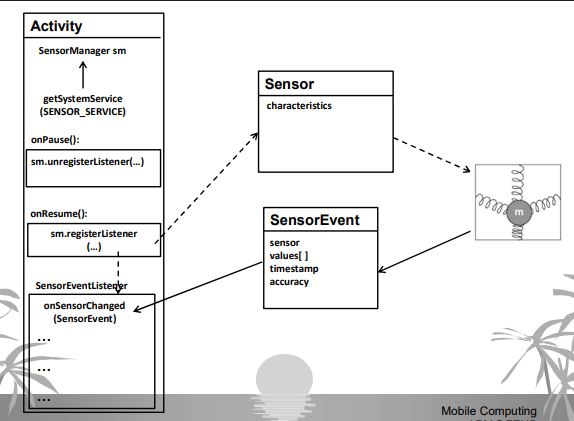
\includegraphics[width=0.8\linewidth]{figures/07_receiving_sensor_measurement.png}
\caption{Receiving sensor measurement}
\label{fig:receiving sensor measurement}
\end{figure}

\subsection{Noise and signal processing}

Many sensors produce several kinds of noise:
\begin{itemize}
    \item High frequency variations with significant amplitudes 
    \item Low frequency deviations (drifts)
\end{itemize} 

Some simple frequency domain filters are useful:

\begin{itemize}
    \item \textbf{Low pass filters}: Weighted smoothing, simple moving average,
simple moving median;
    \item \textbf{High pass filters}: inverse low pass filter;
    \item \textbf{Band pass filters}: Simultaneous low and high pass;
    \item Kalman filters
\end{itemize}






    \section{Lecture 8 - soft keyboard, graphics and media}
    \subsection{Soft keyboard}

Devices can have hard keyboards or only a directional pad (arrows plus select).

Many of the soft keyboard properties can be set from the device 'Settings'. 

However, \texttt{EditText} views can modify the keyboard using the attribute \texttt{android:inputType}. 
It allows different keys (i.e numeric, email, etc.).

Using the attribute \texttt{android:imeOptions} allows different bottom-right keys instead of 'return'.
Example: Next, Send, Done,...

\subsection{Action Events}

Pressing the bottom-right key raises the \texttt{EditorAction} event.
A listener can be defined in \texttt{EditText} views with \texttt{setOnEditorActionListener()}. 

The bottom right menu is a button to show the keyboard, basically.

You can dismiss the keyboard in the handler. By default, the \texttt{Done} key does that. 
Or you can use the code in the handler:

\begin{lstlisting}[title=Code to hide keyboard]
InputMethodManager mgr = (InputMethodManager) getSystemService(INPUT_METHOD_SERVICE);
mgr.hideSoftInputFromWindow(view.getWindowToken(), 0);
\end{lstlisting}

\subsection{2D graphics on the screen - Canvas}
\hl{To draw in android we use the \texttt{Canvas} API}. Canvas API is a drawing 
framework that is provided in Android, with the help of which we 
can create custom shapes like rectangle, circle, and many more 
in our UI design. 

With the help of this API, we can draw any type of shape for 
our app. The drawing of the different shapes is done using Bitmap. 


\begin{figure}[h]
\centering
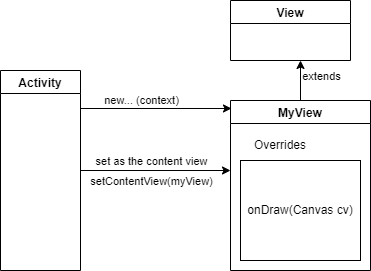
\includegraphics[width=0.7\linewidth]{figures/08_draw_canvas.png}
\caption{Draw Canvas Setup}
\label{fig:draw_canvas}
\end{figure}


The \texttt{Canvas} instance defines a lot of primitives. 
To draw something we use functions like \texttt{draw...}. 
These functions need an instance of \texttt{Paint}. It defines
the characteristics of the drawings, like color, line style and 
width, fonts and sizes, etc. 

Many geometric shapes are defined through a \texttt{Path} instance.
They use the \texttt{canvas.drawPath()} function.

Othre graphic elements are \texttt{Drawable} instances: Bitmaps, 
Shapes, NinePatches, etc. 

Some graphic elements can be defined in xml resources and 
directly used or 'inflated': Colors, Gradients, Shapes, ...


\subsection{Full custom Views}
\hl{This section is mainly an example of how to draw in views.}
Full custom Views need to override several methods from the View
class. 

\begin{itemize}
    \item They can be used in XML layouts;
    \item Parameters from the layout are passed in the
    constructor;
    \item You can create your own event listeners and property
    accessors and modifiers; 
    \item You need to override the \texttt{onMeasure()} method for
    proper behavior, when this View is integrated inside a
    layout; 
    \item You need also to override \texttt{onDraw()} with your
    customized drawing, based on this View properties; 
\end{itemize}

\subsubsection{Example}

\begin{lstlisting}
public class GraphicsView extends View {
    private static final String QUOTE = "Now is the time for all " +
    "good men to come to the aid of their country.";
    private final Path circle;
    private final Paint cPaint;
    private final Paint tPaint;

    public GraphicsView(Context context) {
        super(context);
        circle = new Path();
        circle.addCircle(150, 150, 100, Direction.CW);
        cPaint = new Paint(Paint.ANTI_ALIAS_FLAG);
        cPaint.setStyle(Paint.Style.STROKE);
        cPaint.setColor(Color.LTGRAY);
        cPaint.setStrokeWidth(3);
        tPaint = new Paint(Paint.ANTI_ALIAS_FLAG);
        tPaint.setStyle(Paint.Style.FILL_AND_STROKE);
        tPaint.setColor(Color.BLACK);
        tPaint.setTextSize(20f);
        setBackgroundResource(R.drawable.background);
    }
    @Override
    protected void onDraw(Canvas canvas) {
        canvas.drawPath(circle, cPaint);
        canvas.drawTextOnPath(QUOTE, circle, 0, 20, tPaint);
    }
}
\end{lstlisting}

\begin{lstlisting}
public class Graphics extends Activity {
    @Override
    public void onCreate(Bundle savedInstanceState) {
        super.onCreate(savedInstanceState);
        setContentView(new GraphicsView(this));
    }
}
\end{lstlisting}

\begin{lstlisting}[title=background.xml on res/drawable]
<?xml version="1.0" encoding="utf-8"?>
<shape xmlns:android="http://schemas.android.com/apk/res/android">
<gradient
    android:startColor="#FFFFFF"
    android:endColor="#808080"
    android:angle="270" />
</shape>
\end{lstlisting}

\subsection{Playing audio}
The Android framework encapsulates a complex media player.
Can be used through the framework class \texttt{MediaPlayer}.
\hl{It can work asynchronously} (playing independently of the application) 
and works as a state transition machine object.

Supports a lot of audio formats: wav, aac, mp3, wma, amr (speech), ogg, midi.

For a very simple operation, we must call in order: 
\begin{itemize}
    \item \texttt{release()}: If the object of the MediaPlayer is not null. 
    It is used to release the resources which are associated with MediaPlayer object.
    \item \texttt{create()}: Will create a media player object. We need to specify 
    the resource ID (in res/raw) or a URI: \texttt{mPlayer = MediaPlayer.create(this, R.raw.baitikochi\_chuste);}.
    \item \texttt{start()}: To start playing. It returns immediatly. 
\end{itemize}

\begin{lstlisting}[title=Creates media player on action]
...
@Override
public boolean onKeyDown(int keyCode, KeyEvent event) {
    int resId;
    switch (keyCode) {
        case KeyEvent.KEYCODE_F:
            resId = R.raw.f;
            break;
        default:
            return super.onKeyDown(keyCode, event);
    }

    // Release any resources from previous MediaPlayer
    if (mp != null) {
        mp.release();
    }
    // Create a new MediaPlayer to play this sound
    mp = MediaPlayer.create(this, resId);
    mp.start();
    // Indicate this key was handled
    return true;
}
\end{lstlisting}

\begin{lstlisting}
public class Audio extends Activity {
    private MediaPlayer mp;
    @Override
    public void onCreate(Bundle savedInstanceState) {
        super.onCreate(savedInstanceState);
        setContentView(R.layout.main);
        setVolumeControlStream(
        AudioManager.STREAM_MUSIC);
    }
    ...
}
\end{lstlisting}

\begin{lstlisting}[title=xml]
<LinearLayout xmlns:android=
    "http://schemas.android.com/apk/res/android"
    android:orientation="vertical"
    android:layout_width="fill_parent"
    android:layout_height="fill_parent" >
    <TextView
        android:layout_width="fill_parent"
        android:layout_height="wrap_content"
        android:text="Press the F key"
    />
</LinearLayout>
\end{lstlisting}

\subsection{Playing video}
A video inside a file accessible to your application can be played within a \texttt{VideoView}.

Formats supported include MP4, H.263 (3GP), H.264 (AVC).

Inform the \texttt{VideoView} about the video file path with \texttt{setVideoPath()}.
Start playing with the \texttt{start()} method. 

\hl{Position is not maintained when the device is rotated}. 
Use \texttt{getCurrentPosition()} and save it in \texttt{onSaveInstanceState()}.

Restore the video position with the \texttt{VideoView seekTo()}.

\begin{lstlisting}
public class Video extends Activity {
    @Override
    public void onCreate(Bundle savedInstanceState) {
        super.onCreate(savedInstanceState);
        // Fill view from resource
        setContentView(R.layout.main);
        VideoView video = (VideoView) findViewById(R.id.video);
        // Load and start the movie
        video.setVideoPath("/mnt/sdcard/samplevideo.3gp" );
        video.start();
    }
}
\end{lstlisting}

\begin{lstlisting}[title=XML]
    ...
<FrameLayout
    xmlns:android=
    "http://schemas.android.com/apk/res/android"
    android:layout_width="fill_parent"
    android:layout_height="fill_parent" >
    <VideoView
        android:id="@+id/video"
        android:layout_height="wrap_content"
        android:layout_width="wrap_content"
        android:layout_gravity="center" />
</FrameLayout>

\end{lstlisting}

\begin{lstlisting}[title=Manifest]
...
<activity android:name=".Video"
android:label="@string/app_name"
android:theme=
"@android:style/Theme.NoTitleBar.Fullscreen" >
...
\end{lstlisting}

\subsection{Camera in preview mode}

To display video directly from the camera we need a \texttt{SurfaceView} 
in an \texttt{Activity} layout. 
We need also to orchestrate the camera activation with that \texttt{SurfaceView}
and the \texttt{Activity} life-cycle.

\begin{lstlisting}[title=Steps]
    0. Put a SurfaceView in the Activity layout
    1. [In onCreate()]
    get the SurfaceView from the layout (findViewById())
    get a SurfaceHolder from the SurfaceView (save it on variable)
    add a SurfaceHolder.Callback object (with the callbacks) to the SurfaceHolder
    2. [In onResume()]
    open the Camera (static open() method) and save it
    if the camera was already configured go to 4.
    3. [In the surfaceChanged callback (inside the SurfaceHolder.Callback object)]
    setPreviewDisplay( )
    -- configure the camera
    getParameters()
    -- modify some Parameters
    setParameters()
    4. startPreview() (we see the preview in the screen)
    5. [In onPause()]
    stopPreview()
    release the Camera (release())
\end{lstlisting}


\subsection{3D graphics in Android}

3D graphics are the projection of objects and light on a plane.
The plane is the viewport and is mapped to the screen.

The piece of space projected on the viewport is the
view frustum (a piece of the pyramidal field of view).

\subsubsection{OpenGL}

OpenGL is a big library for 3D graphics programming.
Independent of graphics hardware, designed in 1992 for graphical workstations,
there is a lighter version for mobile devices. 

For using OpenGL ES in Android we use a special view derived from \texttt{GLSurfaceView}.

\begin{figure}[h]
\centering
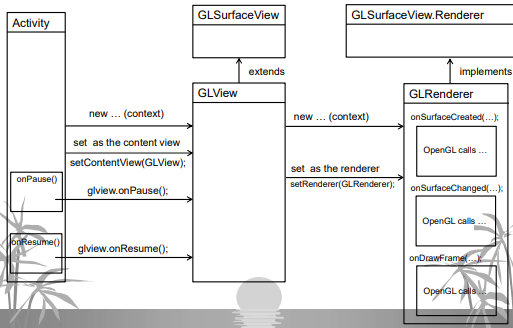
\includegraphics[width=0.8\linewidth]{figures/08_opengl_diagram.png}
\caption{OpenGL diagram}
\label{fig:opengl_diagram}
\end{figure}

% TOUCH EVENTS ========================================================
\subsection{Touch Events}
Many Android devices have only as input the touch screen and gestures.

Many of the events generated by touch are transformed in high level ones like:
\begin{itemize}
    \item Click
    \item LongClick
    \item list item
    \item select
    \item key
\end{itemize}

\hl{But we can intercept them at a lower level using the
\texttt{OnTouchListener} (and its \texttt{onTouch()} method).} 
Since we are in the section about graphics, the touch events 

The \texttt{View} and most of its subclasses generate \texttt{onTouch} events.
Registered with \texttt{setOnTouchListener()}.
When the listener is called it receives the \texttt{View} that caused it and a
\texttt{MotionEvent} instance describing it.

\subsection{MotionEvent}
\texttt{MotionEvent} objects provide information about the touch. 

\begin{itemize}
    \item \texttt{getAction()}: returns in the lower 8 bits a code for theaction: DOWN, UP, MOVE, OUTSIDE, ...
    \item In the higher 8 bits it gives a 'finger' number startingwith 0 (in and after Android 2.2 multitouch issupported).
    \item \texttt{getPointerCount()} returns the number of active 'fingers'.
    \item \texttt{getPointerId(i), getX(i), getY(i)} allows us to extract thenumber and position of each active 'finger'.
\end{itemize}

\begin{lstlisting}[title=Long touch events]
private void dumpEvent(MotionEvent event) {
    String names[] = { "DOWN" , "UP" , "MOVE" , "CANCEL" , "OUTSIDE" ,
    "POINTER_DOWN" , "POINTER_UP" , "7?" , "8?" , "9?" };
    StringBuilder sb = new StringBuilder();
    int action = event.getAction();
    int actionCode = action & MotionEvent.ACTION_MASK;
    sb.append("event ACTION_" ).append(names[actionCode]);
    if (actionCode == MotionEvent.ACTION_POINTER_DOWN || actionCode == MotionEvent.ACTION_POINTER_UP) {
        sb.append("(pid " ).append(action >> MotionEvent.ACTION_POINTER_ID_SHIFT);
        sb.append(")" );
    }
    sb.append("[" );
    for (int i = 0; i < event.getPointerCount(); i++) {
        sb.append("#" ).append(i);
        sb.append("(pid " ).append(
        event.getPointerId(i));
        sb.append(")=" ).append((int) event.getX(i));
        sb.append("," ).append((int) event.getY(i));
        if (i + 1 < event.getPointerCount())
            sb.append(";" );
        }
        sb.append("]" );
        Log.d(TAG, sb.toString());
    }
\end{lstlisting}

\begin{lstlisting}[title=Results]
event ACTION_DOWN[#0(pid 0)=135,179]
event ACTION_MOVE[#0(pid 0)=135,184]
event ACTION_MOVE[#0(pid 0)=144,205]
event ACTION_MOVE[#0(pid 0)=152,227]
event ACTION_POINTER_DOWN(pid 1)[#0(pid 0)=153,230;#1(pid 1)=380,538]
event ACTION_MOVE[#0(pid 0)=153,231;#1(pid 1)=380,538]
event ACTION_MOVE[#0(pid 0)=155,236;#1(pid 1)=364,512]
event ACTION_MOVE[#0(pid 0)=157,240;#1(pid 1)=350,498]
event ACTION_MOVE[#0(pid 0)=158,245;#1(pid 1)=343,494]
event ACTION_POINTER_UP(pid 0)[#0(pid 0)=158,247;#1(pid 1)=336,484]
event ACTION_MOVE[#0(pid 1)=334,481]
event ACTION_MOVE[#0(pid 1)=328,472]
event ACTION_UP[#0(pid 1)=327,471]
\end{lstlisting}


\subsection{Higher level gesteures}

The \texttt{onTouch} listener can pass the \texttt{MotionEventdata} to gesture detectors (Android has two).

\begin{itemize}
    \item \textbf{GestureDetector}: Can detect and trigger events corresponding to one finger gestures.
    Down, Fling, LongPress, Scroll, ShowPress, SingleTap, DoubleTap.
    \item \textbf{ScaleGestureDetector}: Detects the pinch two finger gesture. 
    Generates three events during the gesture: ScaleBegin, Scale, ScaleEnd. 
\end{itemize}



    \section{Lecture 9 - Introduction to flutter}
    \subsection{Widgets}
All the UI in flutter is made by a tree of Widgets. 

Almost all widgets are StatelessWidgets or StatefulWidgets.

\begin{itemize}
    \item immutable;
    \item constructor calls the \texttt{build()} method, that returns the widget;
    \item \texttt{build()} cannot be called again;
    \item new instance must be created in order to redraw the widget;
\end{itemize}

Widgets receive a \texttt{BuildContext} in the \texttt{build()} method .
It is a reference to the location of a Widget in the UI tree and it can contain 
properties concerning the widgets rendering.

\subsection{StatefulWidgets}


\begin{itemize}
    \item Have an associated state object;
    \item State object is mutable and redraws the immutable widget through the \texttt{build()} method;
    \item The \texttt{StatefulWidget} derived class should override at least the 
    \texttt{createState()} method, that returns the associated state object ;
    \item The associated \texttt{State} class should override the \texttt{build()}
    method that returns the \texttt{Widget} (created the first time or redrawn).
\end{itemize}

\begin{lstlisting}
class MyWidget extends StatefulWidget { 
    @override 
    _MyWidgetState createState() => _MyWidgetState(); 
    } 
    
    class _MyWidgetState extends State<MyWidget> { 
    sometype value = initvalue; 
        
    @override Widget build(BuildContext context) { 
        return Container( ...
        // the UI of this widget 
        ); 
    }
}
\end{lstlisting}

\subsubsection{Stateful lifecycle}

\begin{figure}[h]
\centering
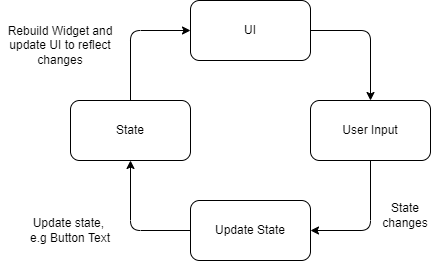
\includegraphics[width=0.8\linewidth]{figures/09_stateful_widget_lifecycle.png}
\caption{Stateful Widget lifecycle}
\label{fig:stateful_widget_lifecycle}
\end{figure}

\begin{itemize}
    \item \texttt{createState()}: Is immediately called after construction;
    \item \texttt{initState()}: Called after creation if overridden; 
    \item \texttt{build()}: To create or redraw a widget tree dependent on the state
    Automatically called if state changes (using \texttt{setState()} or \texttt{didUpdateWidget()});
    \item \texttt{setState()}: Should be called with a function parameter that 
    changes the state and makes a rebuild. 
\end{itemize}

\begin{figure}[h]
\centering
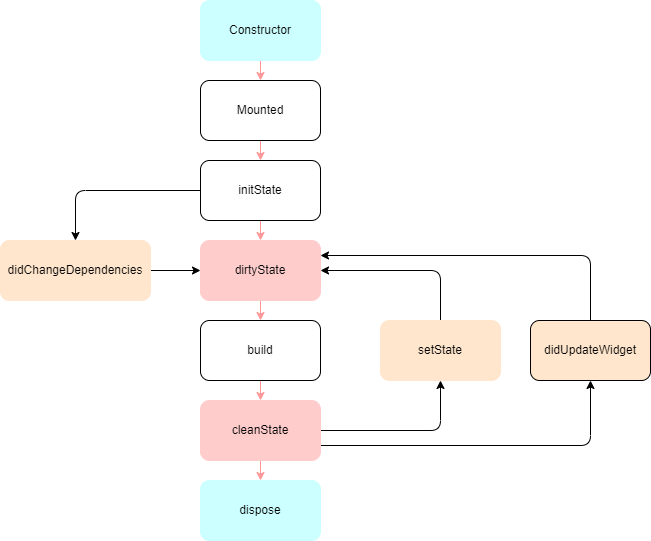
\includegraphics[width=0.8\linewidth]{figures/09_state_object_lifecycle.png}
\caption{State object lifecycle}
\label{fig:state_object_lifecycle}
\end{figure}

\begin{tcolorbox}[colback=red!5,colframe=red!75!black, title=Advantages of stateful widgets over android API]
Supposing that you want to "show a collection of items to a user", or show a list that might be updated, 
in android API, you would have to use an \texttt{ArrayAdapter} or \texttt{BaseAdapter}.  
As explained in the \textbf{Basic Android} chapter, if we want to draw a specific view of the list, we must 
override the ArrayAdapter and create our own view.  

In Flutter, this task is simplified, by using the \texttt{StatefulWidgets}, the collection/list of elements 
is treated as another normal Widget. Everytime the information inside the Widget is updated, it's redrawed 
once again. No overrides are necessary and the code is simplified. 
\end{tcolorbox}





    \section{Lecture 10 - Flutter pages, navigation, drawing and external calls}
    \subsection{Pages}

Page or screen is a Widget tree aka a Route. 

The App widget defines the home route and others, from Home, routes, and initialRoute 
properties (on the App constructor).

The home is the initial screen (widget tree) shown. 
Alternatively, a set of routes (pages) can be defined and an initialRoute specified.

\subsection{Navigation}
The Navigator widget allows the replacement of a page by another using a stack discipline.
It is possible to create a set of navigation routes previously in the app, or build each one
when we want to navigate to it. Initially the App has already a Navigator. We can use it or
create a new independent one with new routes. 

The Navigator defines a set of static methods that manipulate the stack of pages (routes):

\begin{itemize}
    \item \texttt{push(context, Route)} and \texttt{pop(context)}
    \item \texttt{pushName()}, \texttt{removeRoute()}, \texttt{replace()},...
\end{itemize}

\subsubsection{Prebuild route table}
It's possible to prebuild a route table in the App widget and put it in the routes property: 
\begin{lstlisting}
void main() { 
    runApp(MaterialApp( 
        home: MyAppHomePage(), // becomes the route named '/' 
        routes: { 
        '/a': (BuildContext context) => MyPage1(title: 'page A'), 
        '/b': (BuildContext context) => MyPage2(title: 'page B'),   
        '/c': (BuildContext context) => MyPage3(title: 'page C'), }
    ));
    } 
\end{lstlisting}

\subsubsection{Create pages dynamically}
New screens or pages (widgets trees) can be built from a PageRoute (derived from)
e.g., the MaterialPageRoute, requires a WidgetBuilder (a function) that builds the tree
from context. 

\begin{lstlisting}
Navigator.push(context, 
MaterialPageRoute(builder: (context) => MyPage1(title: "page A")));
\end{lstlisting}

\subsubsection{Navigation forward and backward}

\begin{lstlisting}[title=Navigate forward]
// within a widget
... 
Navigator.pushNamed(context, '/b');
\end{lstlisting}

\begin{lstlisting}[title=Navigate backward]
// within the navigated page
...
Navigator.pop(context);
\end{lstlisting}

\subsubsection{Passing data to a route}

\begin{lstlisting}[title=Class to be passed]
class ScreenArguments {
    final String title;
    final String message;
    ScreenArguments(this.title, this.message);
} 
\end{lstlisting}

\begin{lstlisting}[title=Class to create page]
class HomePage extends StatelessWidget {
    @override
    Widget build(BuildContext context) {
        return ...
    ...
    onPressed: () {
        Navigator.pushNamed(context, '/page2',
        arguments: ScreenArguments('Title', 'Message'));
    }
    ...
    }
}
\end{lstlisting}

\begin{lstlisting}[title=Page]
// App root widget
...
return MaterialApp(
    routes: { '/page2': (context) => SecondPage() },
    home: HomePage() // route name: '/'
)
...
class SecondPage extends StatelessWidget {
    @override
    Widget build(BuildContext context) {
        final ScreenArguments args = ModalRoute.of(context).settings.arguments;
        return ...
            ... args.title ...
            ... args.message ...
    }
}
\end{lstlisting}

\subsubsection{Return a value using pop}
When we do a \texttt{Navigator.pop(context)}, \texttt{pop()} accepts a second parameter that is a
result. It can be of any type.

This result is returned by the \texttt{Navigator.push(...)} that created the popped page.
The result comes in a \texttt{Future}, resolved only when the page is popped.

\begin{lstlisting}[title=Example]
// caller 
final result = await Navigator.push(context, MaterialPageRoute(builder: (context) => SomePage())); 

// New page - SomePage
Navigator.pop(context, 'Some message');
\end{lstlisting}


\subsection{External HTTP Calls}
Flutter does not have a direct API for web requests.
But there are several packages in the package repository (pub.dev).

One of the simplest is the http package (https://pub.dev/packages/http)
For using external packages, it is necessary to import them in code, and to
declare them in the project pubspec.yaml file. Finally, it must be downloaded.

\begin{tcolorbox}
The declaration and installation can be done from the command line, or from the
used IDE:

\texttt{\$ flutter pub add http}
\end{tcolorbox}

For example, to define a function to perform a REST GET request:

\begin{lstlisting}
    import 'package:http/http.dart';
    ...
    Future<String> getResponse() async {
    final response = await http.get(Uri.http('data.fixer.io', '/api/latest',
        { 'access_key': '<your API key>',
            'base': 'EUR',
            'symbols': 'USD,GBP' 
        }
    ));
    if (response.statusCode == 200)
        return response.body;
    else
        throw Exception('HTTP failed');
    }
\end{lstlisting}

    \section{Lecture 11 - Flutter app architecture}
    \subsection{MVC's architecture}
The MVC architecture holds:
\begin{itemize}
    \item \textbf{Models} - Holds the application state and simple operations to access/filter/manipulate
    that data. These operations are also called the Domain Logic.
    \item \textbf{Views} - the UI and pages build with the Flutter widgets. This layer may also contain the
    "view controllers" with handlers for local interactions.
    \item \textbf{Controller} - contains the Application Logic composed by the business operations that
    constitute the functionalities of the application. These operations can be organized in \textbf{Commands}
    invoked by the other layers, but mainly is result of UI interactions.
    \item \textbf{Services} - contain the operations in the outside world. Usually, they are invoked by
    Commands that can retrieve data and inject it on Models, or in the other direction.
\end{itemize}

\begin{figure}[h]
\centering
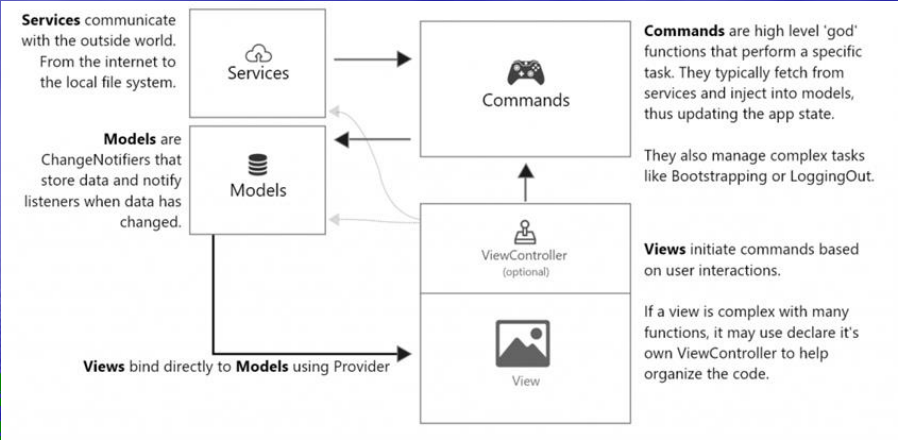
\includegraphics[width=0.8\linewidth]{figures/11_MVC_diagram.png}
\caption{MVC diagram}
\label{fig:mvc_diagram}
\end{figure}
\newpage
The implementation of this architecture requires access to the \texttt{Models} in every place in
the App. For doing that, a special widget is provided in an external package. It associates
\texttt{Models} and \texttt{Services} with the application context. The package is called \texttt{Provider}. 


\begin{figure}[h]
\centering
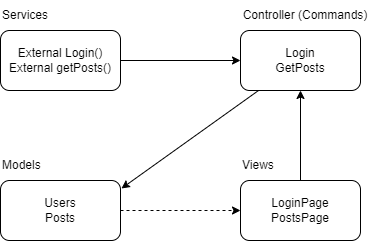
\includegraphics[width=0.6\linewidth]{figures/11_mvc_example_diagram.png}
\caption{MVC diagram example}
\label{fig:mvc_diagram_example}
\end{figure}

\subsection{Redux Architecture}
The Redux architecture specifies that all the application state is centralized in the
Store block (it can contain several Models). is a state management architecture library 
that successfully distributes data across widgets in a repetitive 
manner. It manages the state of an application through a unidirectional flow of data.

\begin{figure}[h]
\centering
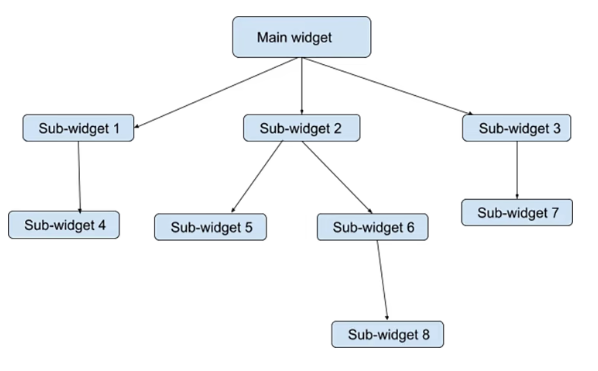
\includegraphics[width=0.4\linewidth]{figures/11_flow_data.png}
\caption{An unidirectional flow of data}
\label{fig:flow_data}
\end{figure}
In this example, data generated in the main widget is needed in sub-widget 8. 
Ordinarily, this data passes through sub-widget 2 to sub-widget 6 and then, finally, 
it reaches sub-widget 8. This is also the case for widgets that need data 
generated or saved in the state of any widget that's higher up in the hierarchy.

With Redux, \hl{you can structure your application so that the state is extracted in 
a centrally-located store. The data in this centralized store can be accessed 
by any widget that requires the data, without needing to pass through a chain of 
other widgets in the tree.}

Any widget that needs to add, modify, or retrieve the data in a state managed by the 
Redux store would have to request it with the appropriate arguments.

Likewise, for every change made to the state, the dependent widgets respond to the change 
either through the user interface or any other configured means.

\subsubsection{Why is it important?}
In a medium or large-scale application with many widgets, when a child widget needs data, 
it is common to manage the data from the main.dart file.

This data could be distributed through the constructors of widgets as arguments 
until the data gets to the recipient widget, 
\hl{this could lead to a long chain of data transfer through widgets that don't need this data.}

Not only can it be cumbersome and difficult to pass data through the constructors, 
\hl{it can also affect the performance of an application. This is because when you manage 
data from the main widget - or any root widget - the entire widget tree rebuilds 
whenever a change occurs in any of its child widgets}. You only want to run the 
build method in the widget that requires the changed data.

\subsubsection{How it works}
In Redux there's a \texttt{Store} which holds a \texttt{State} object that represents the 
\hl{state of the whole application}. Every application event (either from the user or external) 
is represented as an \texttt{Action} that gets dispatched to a \texttt{Reducer} function. 
This \hl{\texttt{Reducer} updates the \texttt{Store} with a new \texttt{State} depending on 
what \texttt{Action} it receives}.  
And whenever a new \texttt{State} is \hl{pushed (the state is immutable, thus it can't be 
modified, just replaced)}  through the \texttt{Store} the \texttt{View} is recreated to reflect 
the changes.

With Redux most components are decoupled, making UI changes very easy to make.
 In addition, the only business logic sits in the \texttt{Reducer} functions. 
 A \texttt{Reducer} is a function that takes an \texttt{Action} and the current application
  \texttt{State} and it returns a \hl{new} \texttt{State} object, therefore it is straightforward 
  to test because we can write a unit test that sets up an initial State and checks that 
  the \texttt{Reducer} returns the new and modified \texttt{State}.

\subsubsection{Middleware}
what happens when the application has to perform some asynchronous operation, such as 
loading data from an external API? This is why people came up with a new component
 known as the \texttt{Middleware}.

\texttt{Middleware} is a component that may process an \texttt{Action} before 
it reaches the \texttt{Reducer}. It receives the current application \texttt{State}
 and the \texttt{Action} that got dispatched, and it can run some code 
 (usually a side effect), such as communicating with a 3rd-party API or data source. 
 Finally, the \texttt{Middleware} may decide to dispatch the original \texttt{Action}, 
 to dispatch a different one, or to do nothing more. 
 
\subsubsection{Resume according to slides}
The \texttt{View} (flutter widget tree) generates \texttt{Actions} from user interactions, that specify
external requests and/or state modifications. The external requests are filtered out
by a \texttt{Middleware} block. The other \texttt{Actions} go to a \texttt{Reducer} function.

The \texttt{Reducer} function modifies the Store, according to the specified \texttt{Action}.
\texttt{Views} have access to the \texttt{Store}, and whenever this is modified it triggers a \texttt{View}
redrawing, taking into account the app state inside the \texttt{Store}.

\begin{figure}[h]
\centering
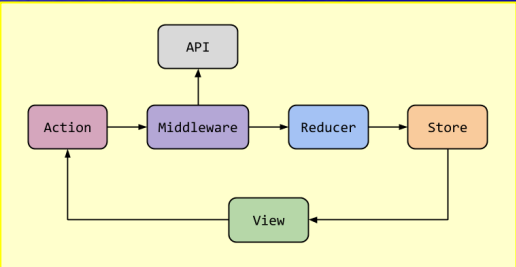
\includegraphics[width=0.8\linewidth]{figures/11_redux_diagram.png}
\caption{Redux architecture diagram}
\label{fig:redux_architecture_diagram}
\end{figure}

    \newpage
    \section{Lecture 12 - Flutter native channels}
    We can use a function called \texttt{invokeMethod('method\_name', parameters)} to 
call native functions from a specific system. 

\begin{lstlisting}
const channel = MethodChannel('API_name');
final ResultType response = await channel.invokeMethod('method\_name', parameters);
\end{lstlisting}

The channel can also define Callback methods to be called from native code.

\subsection{Catching native events}
Can be done using an \texttt{EventChannel} between the Dart side and the native side.

On the Dart side a receiver should be established defining callbacks called when an
event is generated in the native side.

The native side establishes a \texttt{StreamHandler} attached to the channel, together with an
\texttt{EventSink}, capable of generating events that can carry data. It's possible to also
generate error events.

The appropriate Dart side callback is called whenever an event is generated.


    \section{Lecture X - MVVM}
    Model-view-viewmodel (MVVM) is a software that helps to 
cleanly separate business and presentation logic of an
application from the its user interface (UI), \hl{making it
easier to test, maintain and evolve}. It can also \hl{code re-use}
opportunities and allows developers and UI designers to more 
\hl{easily collaborate} when developing their respective parts 
in the app. This is a famous pattern and used in \hl{Xamarim} and 
it is similar to the \textbf{MVP} (Model View Presenter) pattern, however
the drawbacks of the MVP has been solved.

\subsection{The MVVP Pattern}
The pattern is divided in three parts: the model, the view and the 
view model. 

\begin{figure}[h]
\centering
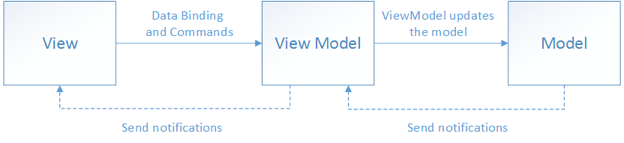
\includegraphics[width=0.8\linewidth]{figures/13_mvvm.png}
\caption{The MVVM pattern}
\label{fig:mvvm_pattern}
\end{figure}


At a high level, the view "knows about" the view model, 
and the view model "knows about" the model, but the model 
is unaware of the view model, and the view model is unaware 
of the view. Therefore, the view model isolates the view from 
the model, and allows the model to evolve independently of the view.


The separate code layers of MVVM are:
\begin{itemize}
    \item \textbf{Model}: this layer is responsible for the abstraction of the 
    data sources. Model and ViewModel work together to get and save the data.
    \item \textbf{View}: The purpose of this layer is to inform the ViewModel 
    about the user's action. This layer observes the ViewModel and does 
    not contain any kind of application logic.
    \item \textbf{ViewModel}:  It exposes those data streams which are relevant to 
    the View. Moreover, it serve as a link between the Model and the View.
\end{itemize}
\subsection{Advantages and disadvantages}
\textbf{Advantages:}
\begin{itemize}
    \item Enhance the reusability of code.
    \item All modules are independent which improves the testability of each layer.
    \item Makes project files maintainable and easy to make changes.
\end{itemize}

\textbf{Disadvantages}:
\begin{itemize}
    \item This design pattern is not ideal for small projects.
    \item If the data binding logic is too complex, the application 
    debug will be a little harder.
\end{itemize}

\subsection{Implementation and DataBinding}
There are 2 ways to implement MVVM design pattern in Android projects:
\begin{itemize}
    \item Using the \hl{DataBinding} library released by Google.
    \item Using any tool like RxJava for DataBinding. 
\end{itemize}

Google releases the Data Binding Library for Android that allows the developers 
to bind UI components in the XML layouts with the application's data repositories. 
This helps in minimizing the code of core application logic that binds with View. 
Further, Two - way Data Binding is done for binding the objects to the XML layouts 
so that object and the layout both can send data to each other. 




 
    \section{Resources}
    IOC: https://www.sitepoint.com/three-design-patterns-that-use-inversion-of-control/  \\
    Threads: https://www.oreilly.com/library/view/efficient-android-threading/9781449364120/ch04.html  \\
    Audio Media: https://www.tutlane.com/tutorial/android/android-audio-media-player-with-examples \\ 
    Canvas API: https://www.geeksforgeeks.org/how-to-use-canvas-api-in-android-apps/ \\ 
    Xamarim MVVM: https://docs.microsoft.com/en-us/xamarin/xamarin-forms/enterprise-application-patterns/mvvm \\ 
    Xamarim MVVM: https://www.geeksforgeeks.org/mvvm-model-view-viewmodel-architecture-pattern-in-android/ \\ 
    Reducer: https://blog.logrocket.com/flutter-redux-complete-tutorial-with-examples/ \\ 
\end{document}  

% ---------------------
% Bibliography
% --------------------- 
% A folder bst/report.bib should be created 
\bibliographystyle{unsrt}
\bibliography{bst/report}  


